\documentclass[10pt]{beamer}
\usetheme[progressbar=foot]{metropolis}           % Use metropolis theme

\usepackage{graphicx}
\graphicspath{ {./images/} }

\usepackage[style=authortitle,backend=biber,sorting=none]{biblatex}
\bibliography{references}

\title{Interview at Diamond Light Source}
\date{13\textsuperscript{th} February 2024}
\author{Dr Matthew Heath}
\subtitle{For the position of Senior DevOps Engineer}
\titlegraphic{\flushright
\includegraphics[width=4cm]{diamond-logo}}

\begin{document}
  \maketitle
  \begin{frame}{Table of Contents}
    \tableofcontents
  \end{frame}

  \section{Career Highlights}
  \begin{frame}{Overview}
    \begin{columns}
      \column{0.5\textwidth}
        \begin{itemize}
          \item \textbf{Doctoral Student}
          \\\alert{University of Edinburgh}
          \\(Sept 2016 -- Feb 2022)
          \item \textbf{Storage System Administrator}
          \\\alert{STFC}
          \\(Jan 2021 -- May 2022)
          \item \textbf{Cloud Engineer}
          \\\alert{EscherCloud}
          \\ (Jun 2022 -- Jan 2024)
        \end{itemize}

      \column{0.5\textwidth}
        \begin{columns}
          \column{0.5\textwidth}
            
\includegraphics[width=0.9\textwidth]{uoe-logo}\\
            \vspace{0.5cm}
            
\includegraphics[width=0.9\textwidth]{cern-logo}
          \column{0.5\textwidth}
            
\includegraphics[width=0.8\textwidth]{eschercloud-logo}\\
            \vspace{0.75cm}
            
\includegraphics[width=0.9\textwidth]{stfc-logo}
        \end{columns}        
    \end{columns}
  \end{frame}

  \section{CERN and the University of Edinburgh}
  \begin{frame}{Doctoral Student}
    \begin{columns}
      \column{0.6\textwidth}
        \begin{itemize}
          \item Conducted research as a member of the ATLAS Experiment.
          \footcite{thesis}
          \item Emulated complex detector geometry as part of \textsc{FastCaloSim}
          upgrade. \footcite{atlfast3}
          \item ML derived multivariate reweightings of simulation samples.
          \footcite{hgamgam}
        \end{itemize}

      \column{0.4\textwidth}
        
\includegraphics[width=0.8\textwidth, angle=25]{thesis}\\
        \vspace{0.5cm}
        
\includegraphics[width=2cm]{atlas-logo}
    \end{columns}
  \end{frame}

  \section{Science and Technology Facilities Council}
  \begin{frame}{Storage System Administrator}
    \begin{itemize}
      \item Maintained and developed 24/7 availability storage services for the
      Data Services group in the Scientific Computing Department.
      
      \item Managed key storage services:
        \begin{itemize}
          \item \textbf{Echo:} $\sim$70PiB Ceph object store.
          \item \textbf{Deneb:} $\sim$4PiB Ceph file system.
          \item \textbf{Sirius:} $\sim$700TiB Ceph block store
          backend for the Cinder service of SCD's OpenStack cloud platform.
        \end{itemize}
  
      \item Provided line management and mentoring:
        \begin{itemize}
          \item Mentored members of the internship program.
          \item Guided junior members of the storage team.
        \end{itemize}
  
      \item Conducted Research and Development:
        \begin{itemize}
          \item Explored prospective new services and developments in the
          storage domain.
        \end{itemize}
  
      \item On-call Support:
        \begin{itemize}
          \item Part of the on-call rota for addressing service issues outside
          of office hours.
        \end{itemize}
    \end{itemize}
  \end{frame}

  \begin{frame}{VOMS AuthN/AuthZ for Echo}
    \begin{itemize}
      \item \textbf{Objective:} Strengthen security and access control for
      Echo object store service via the XRootD protocol.
  
      \item \textbf{Previous AuthN/AuthZ Process:}
        \begin{itemize}
          \item AuthN: VOMS certificate.
          \item AuthZ: Scheduled lookup file update based on virtual organisation
          databases.
        \end{itemize}
  
      \item \textbf{Challenges:}
        \begin{itemize}
          \item Delayed permissions updates posed security risks.
          \item Potential access for recently rescinded users during updates.
        \end{itemize}
  
      \item \textbf{Implemented Solution:}
        \begin{itemize}
          \item Configured XRootD authZ/N to directly integrate with virtual
          organisation VOMS servers.
          \item Real-time access to the latest object, role, and member permissions.
          \item Provided SCD admins with utility for custom banlist curation.
        \end{itemize}
  
      \item \textbf{Outcome:}
        \begin{itemize}
          \item Enhanced security and access control for Echo object store service.
          \item Mitigated risks of delayed updates and unauthorised access.
        \end{itemize}
    \end{itemize}
  \end{frame}

  \section{EscherCloud}
  \begin{frame}{Cloud Engineer}
    \begin{itemize}
      \item \textbf{EscherCloud:} Startup providing GPU-enabled
      private cloud services, emphasising sustainability, European data sovereignty,
      and democratising AI/ML.
  
      \item \textbf{Role and Achievements:}
        \begin{itemize}
          \item Deployed and managed Ceph storage backend for OpenStack, forming
          the foundation for the inaugural PaaS offering.
          \item Expanded responsibilities to encompass all aspects of cloud
          infrastructure, from server provisioning to monitoring, visualisation,
          and central logging.
          \item Managed OpenStack services, VLANs, DNS, private network access,
          and more.
        \end{itemize}
  
      \item \textbf{Contributions to Company Growth:}
        \begin{itemize}
          \item Enabled onboarding of engineering interns, providing ongoing
          line management and mentoring as they transitioned to full employees.
        \end{itemize}
    \end{itemize}
  \end{frame}

  \begin{frame}{Configuration Management Automation}
    \begin{itemize}
      \item \textbf{Overview:} Developed a comprehensive configuration automation
      service, unifying server inventory with a CIDB.
  
      \item \textbf{Ansible Implementation:}
        \begin{itemize}
          \item Utilised CIDB API for real-time physical and virtual server inventory.
          \item Implemented Ansible plugin for up-to-date playbooks based on server
          inventory groupings.
        \end{itemize}
  
      \item \textbf{Rundeck Deployment:} Implemented Rundeck for a streamlined UI,
      codifying and simplifying automation job execution.
  
      \item \textbf{Benefits:}
        \begin{itemize}
          \item Achieved efficient and centralised infrastructure configuration
          management.
          \item Simplified automation job execution through Rundeck.
        \end{itemize}
    \end{itemize}
  \end{frame}

  \begin{frame}{VM System Backup Service}
    \begin{itemize}
      \item \textbf{Overview:} Developed a backup tool for libvirt KVMs across
      a data centre.
  
      \item \textbf{Key Features:}
        \begin{itemize}
          \item Utilised restic, a modern backup program written in Go, for
          secure backups to Ceph S3 object storage.
          \item Deployed Ansible for automation and developed custom Python
          modules for Virsh libvirt interaction.
        \end{itemize}
  
      \item \textbf{Custom Ansible Modules:}
        \begin{itemize}
          \item Developed custom Python modules to interface with the Virsh
          libvirt command line tool.
          \item Extracted full KVM specifications and managed virtual disk
          images for seamless data export without downtime.
        \end{itemize}
  
      \item \textbf{Benefits:}
        \begin{itemize}
          \item Established a robust backup solution, ensuring data integrity
          and efficient recovery.
          \item Utilised restic and Ceph S3 for streamlined backup processes.
        \end{itemize}
    \end{itemize}
  \end{frame}

  \begin{frame}{Zero Trust Access Control Plane}
    \begin{itemize}
      \item \textbf{Overview:} Implemented zero-trust access for EscherCloud admins
      and engineers.
  
      \item \textbf{Zero-Trust Definition:} A security model demanding strict
      identity verification for resource access, irrespective of network location.
      No default trust in users or systems.
  
      \item \textbf{Tool Assessment:} Explored Pomerium, TailScale, and Warpgate
      as possible access solutions, selecting Teleport.
  
      \item \textbf{Teleport Features:} Provided secure and configurable MFA, RBAC,
      and IDAC for server access, extending benefits to a secure reverse proxy for
      private network web applications. Also provided implementation of machine users
      to provide access for service accounts like an Ansible user.
  
      \item \textbf{Benefits:} Implemented a robust zero-trust approach for heightened
      security, leveraging Teleport for enhanced access control and web service
      security.
    \end{itemize}
  \end{frame}

  \section{Interests and Hobbies}
  \begin{frame}{\`A la Cuisine}
    \begin{columns}
      \column{0.33\textwidth}
        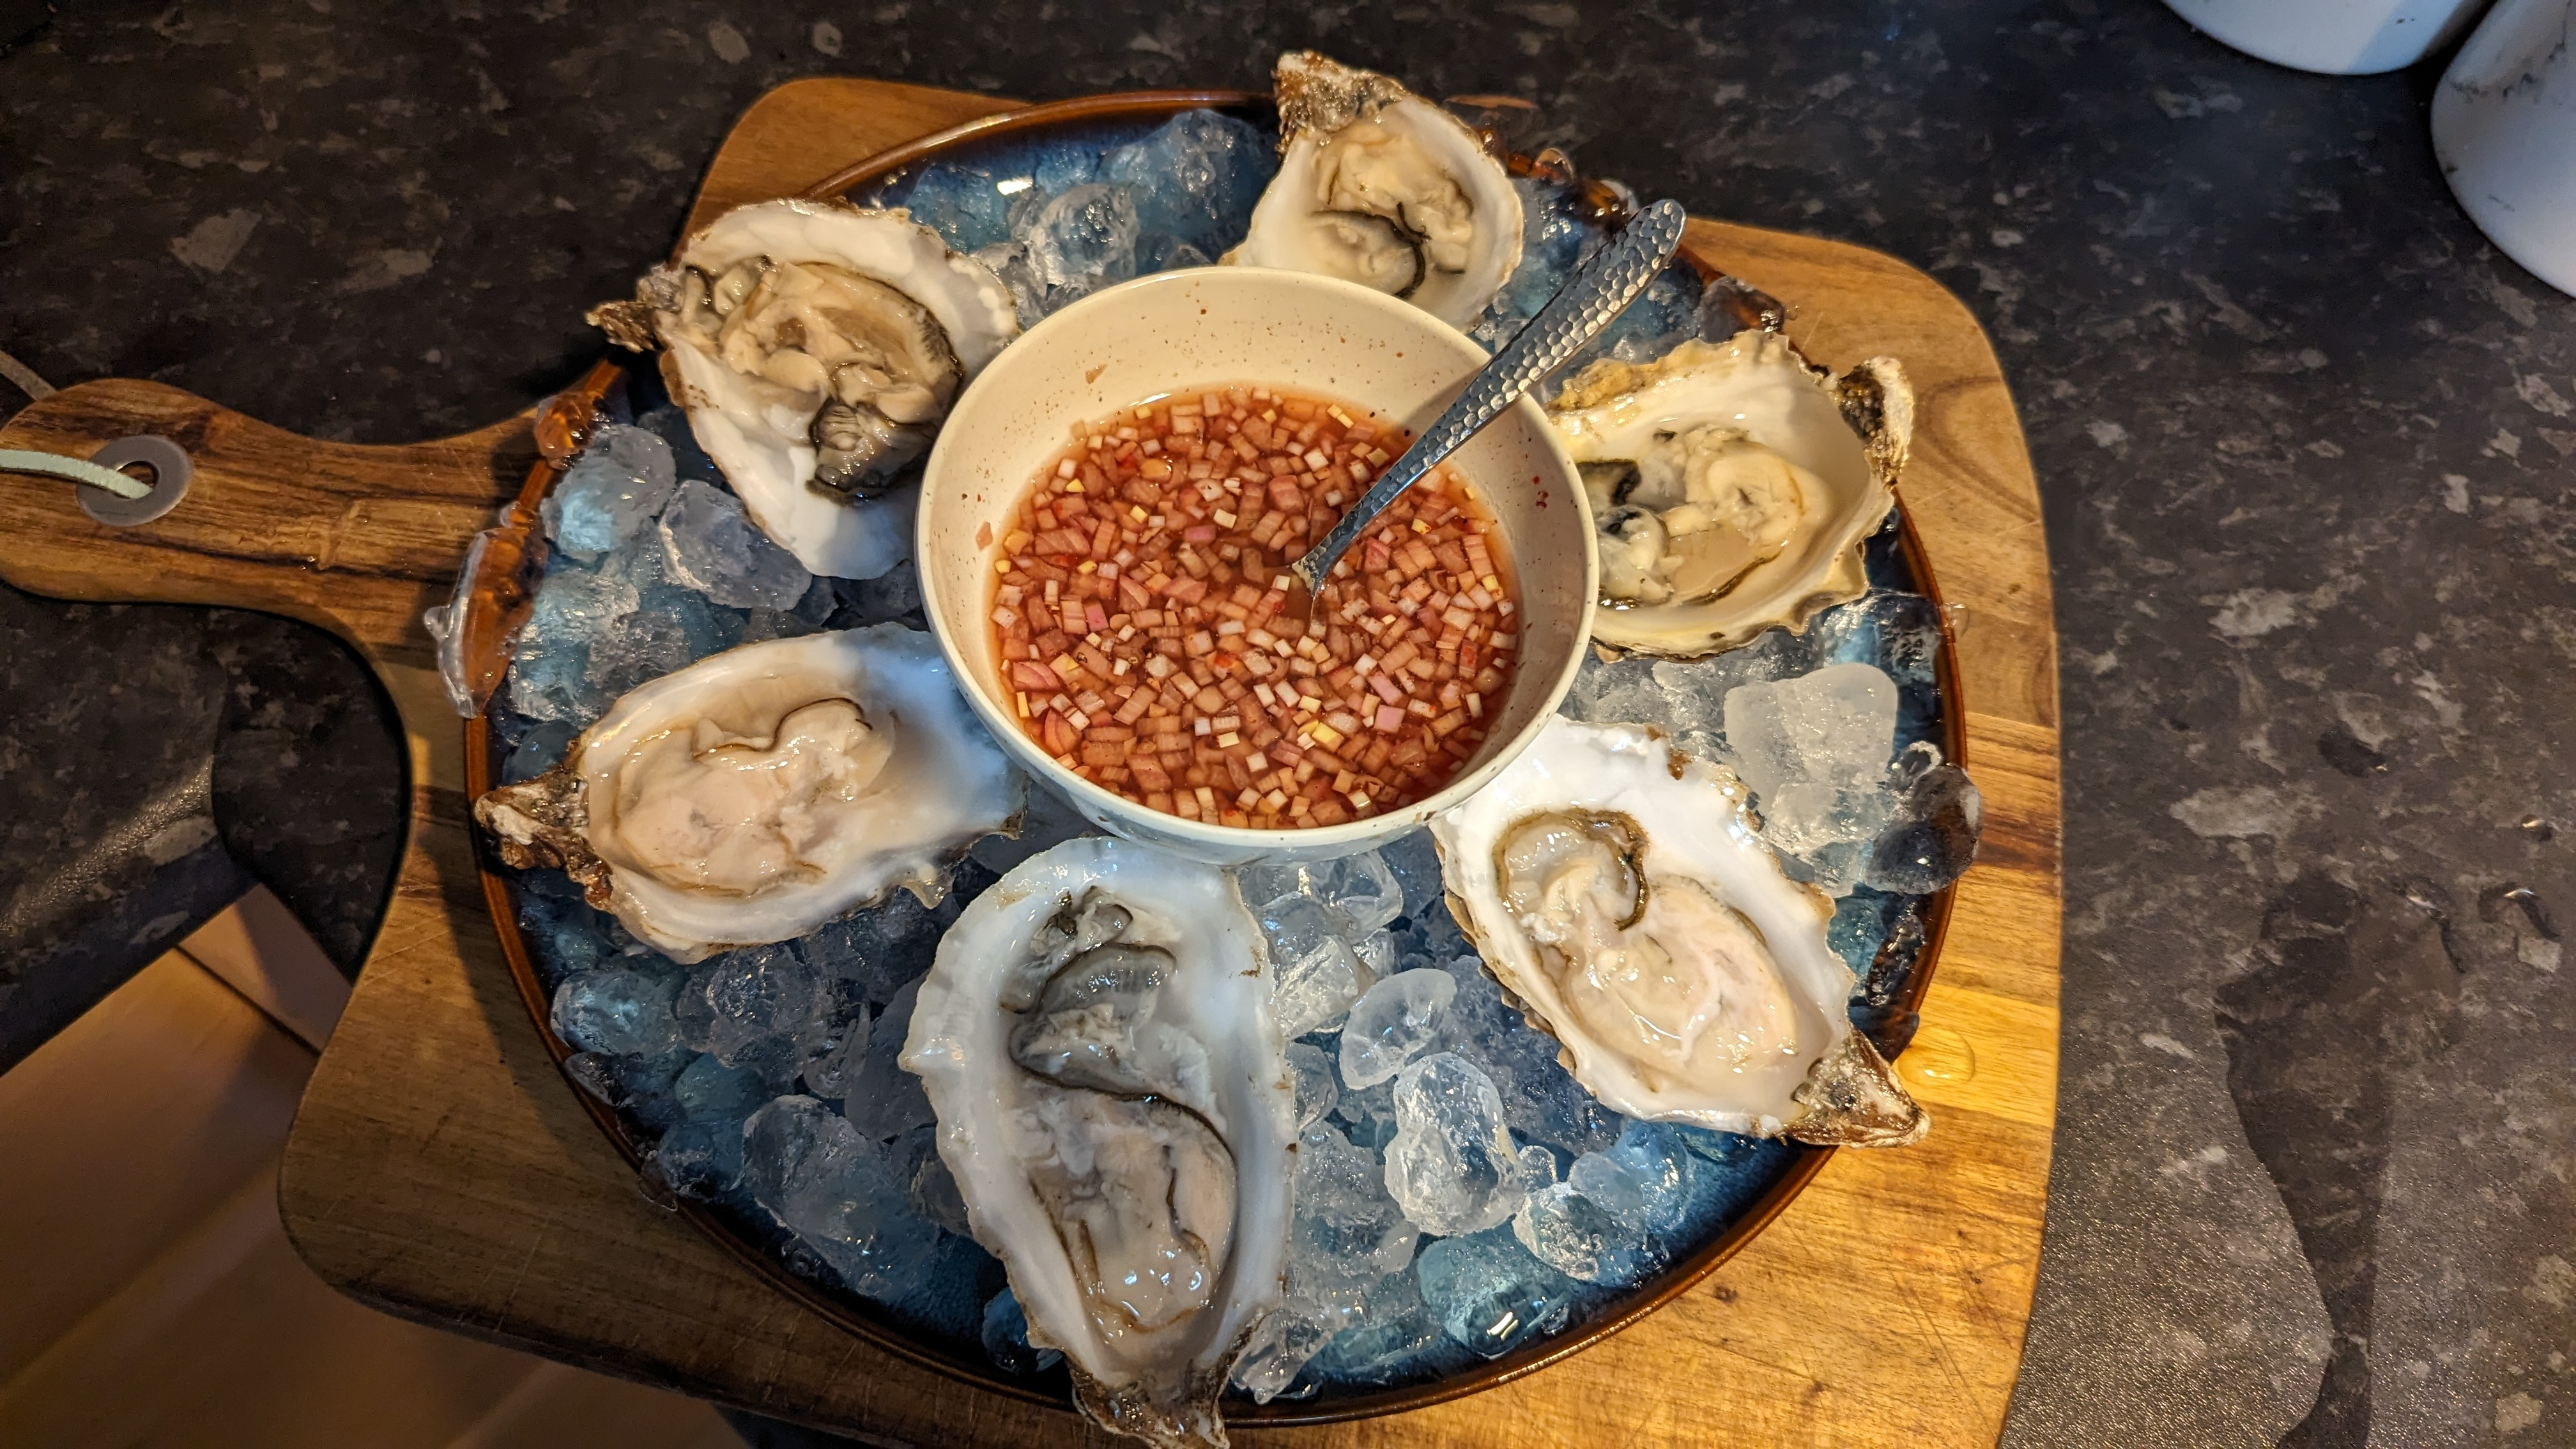
\includegraphics[width=\textwidth]{oysters}\\
        \vspace{0.2cm}
        \includegraphics[width=\textwidth]{steak}\\
        \vspace{0.2cm}
        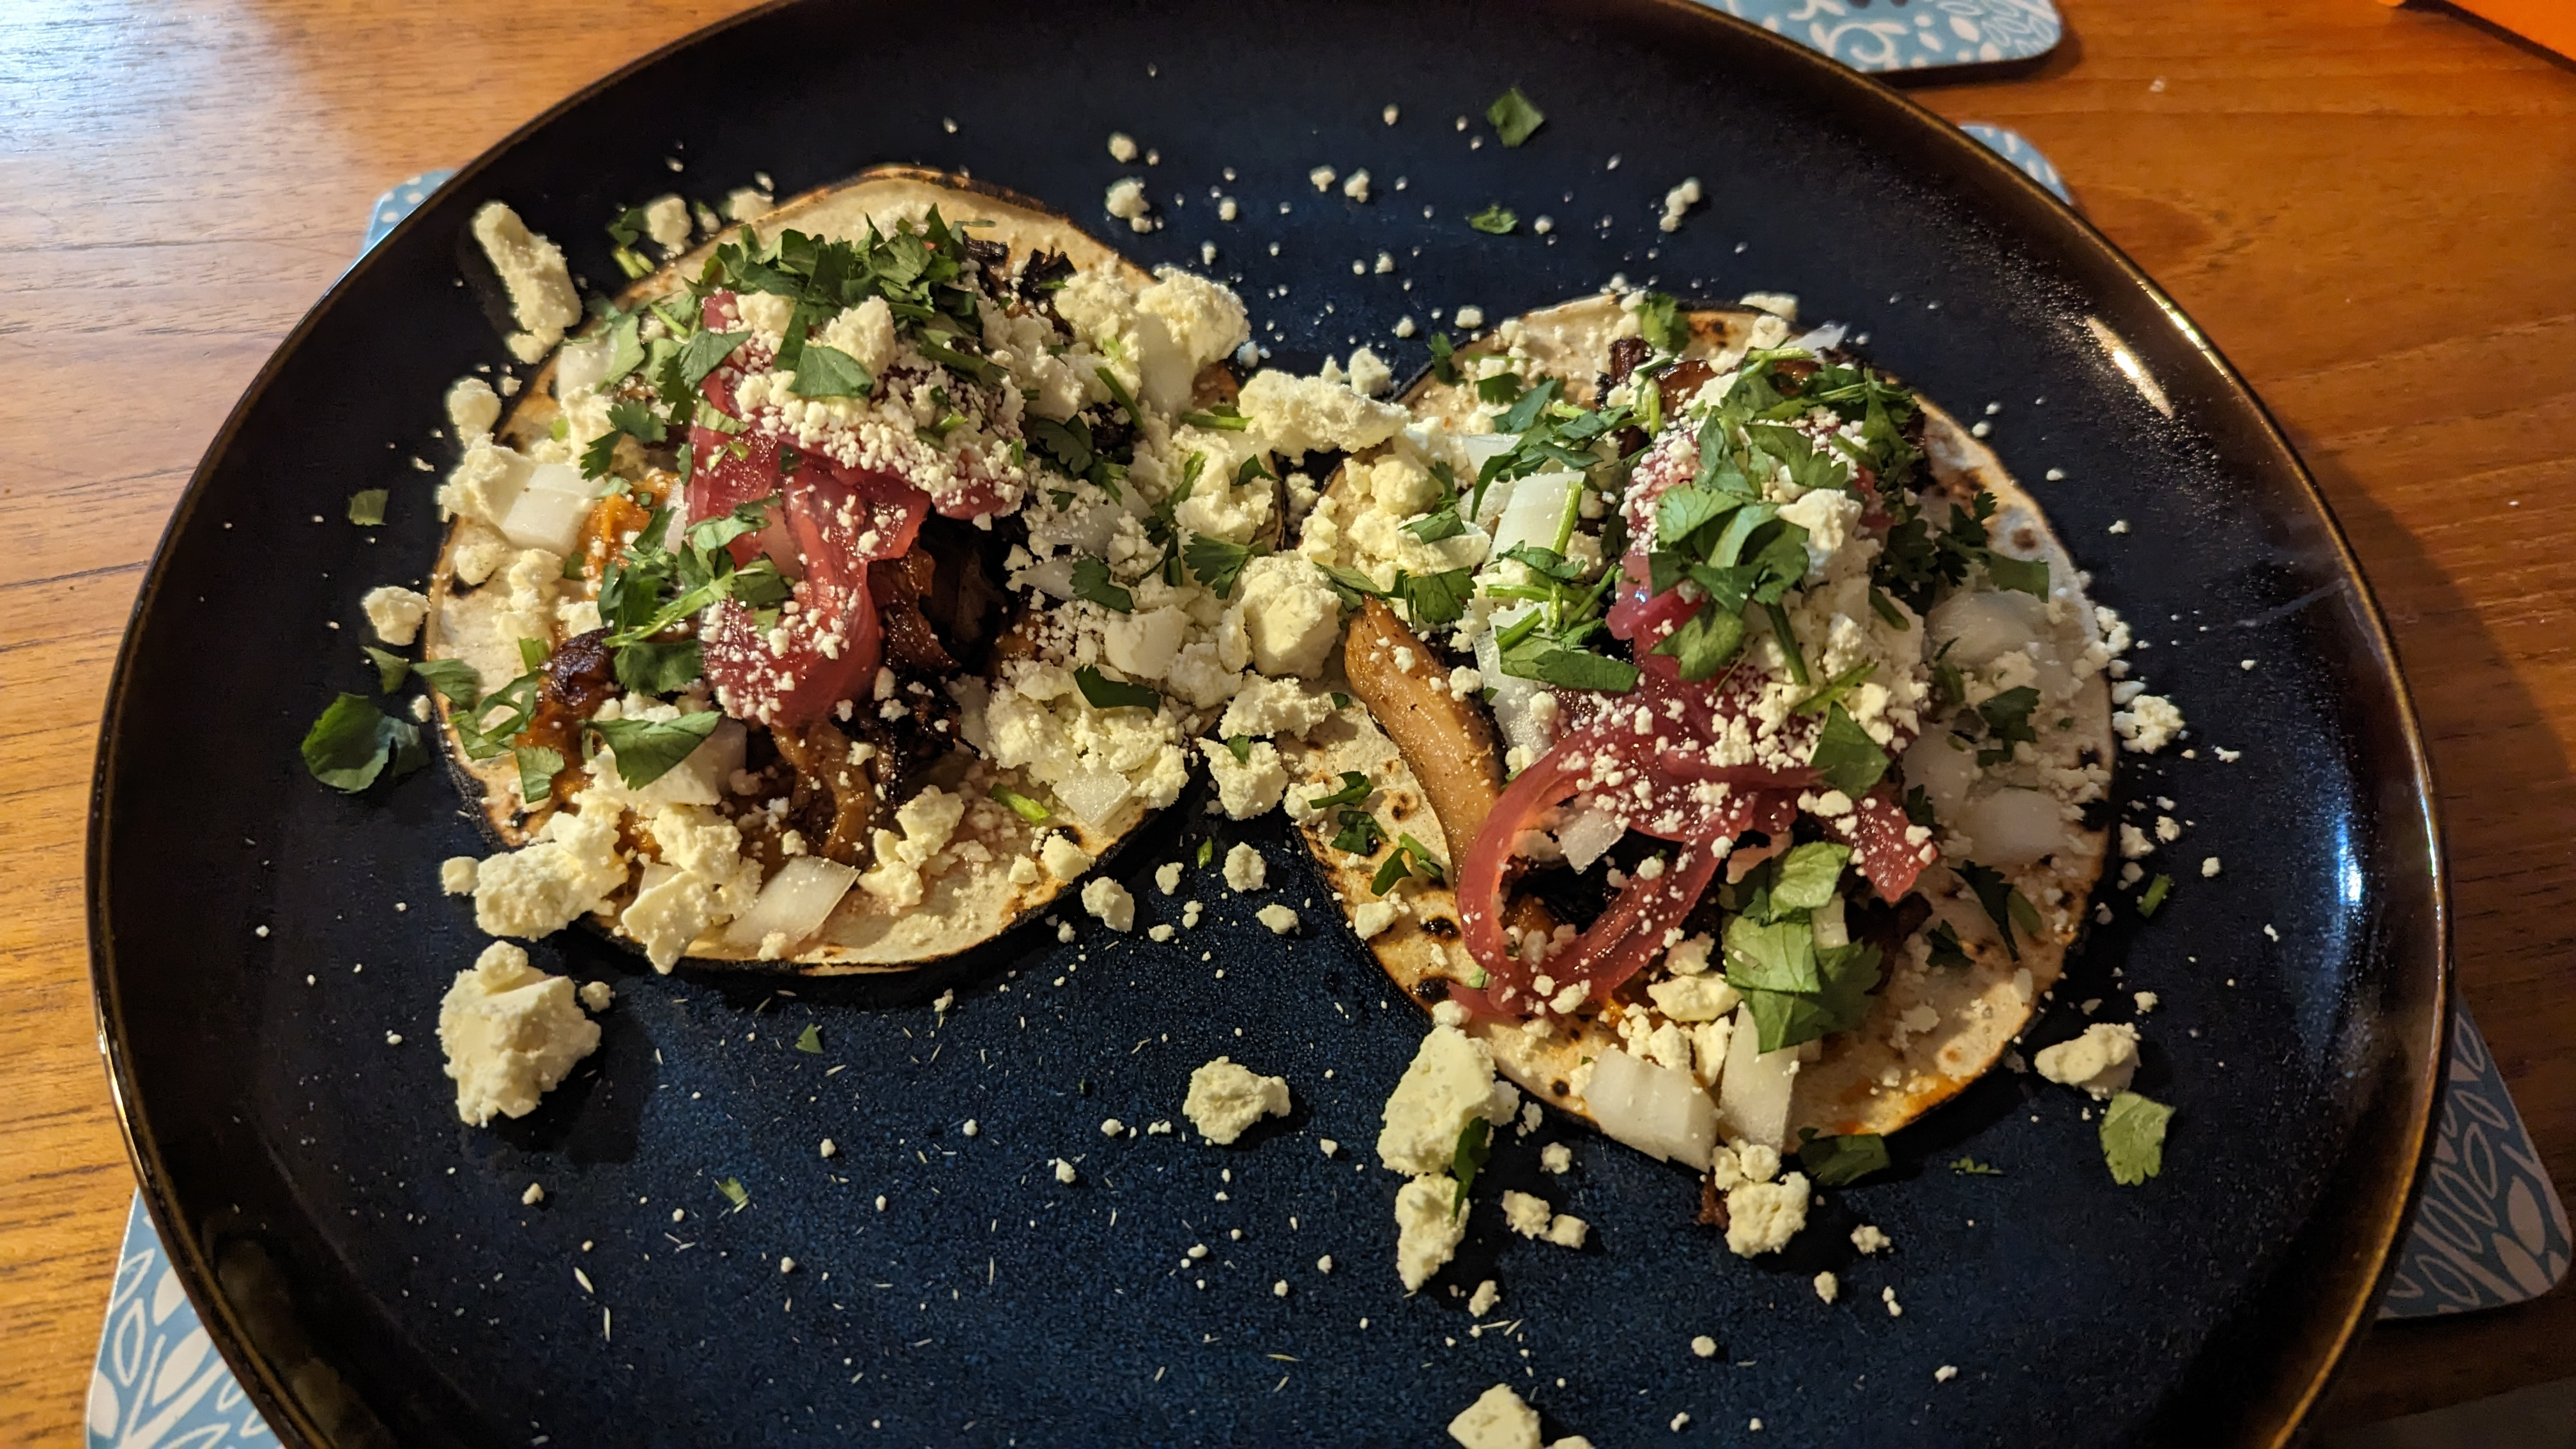
\includegraphics[width=\textwidth]{tacos}

      \column{0.33\textwidth}
        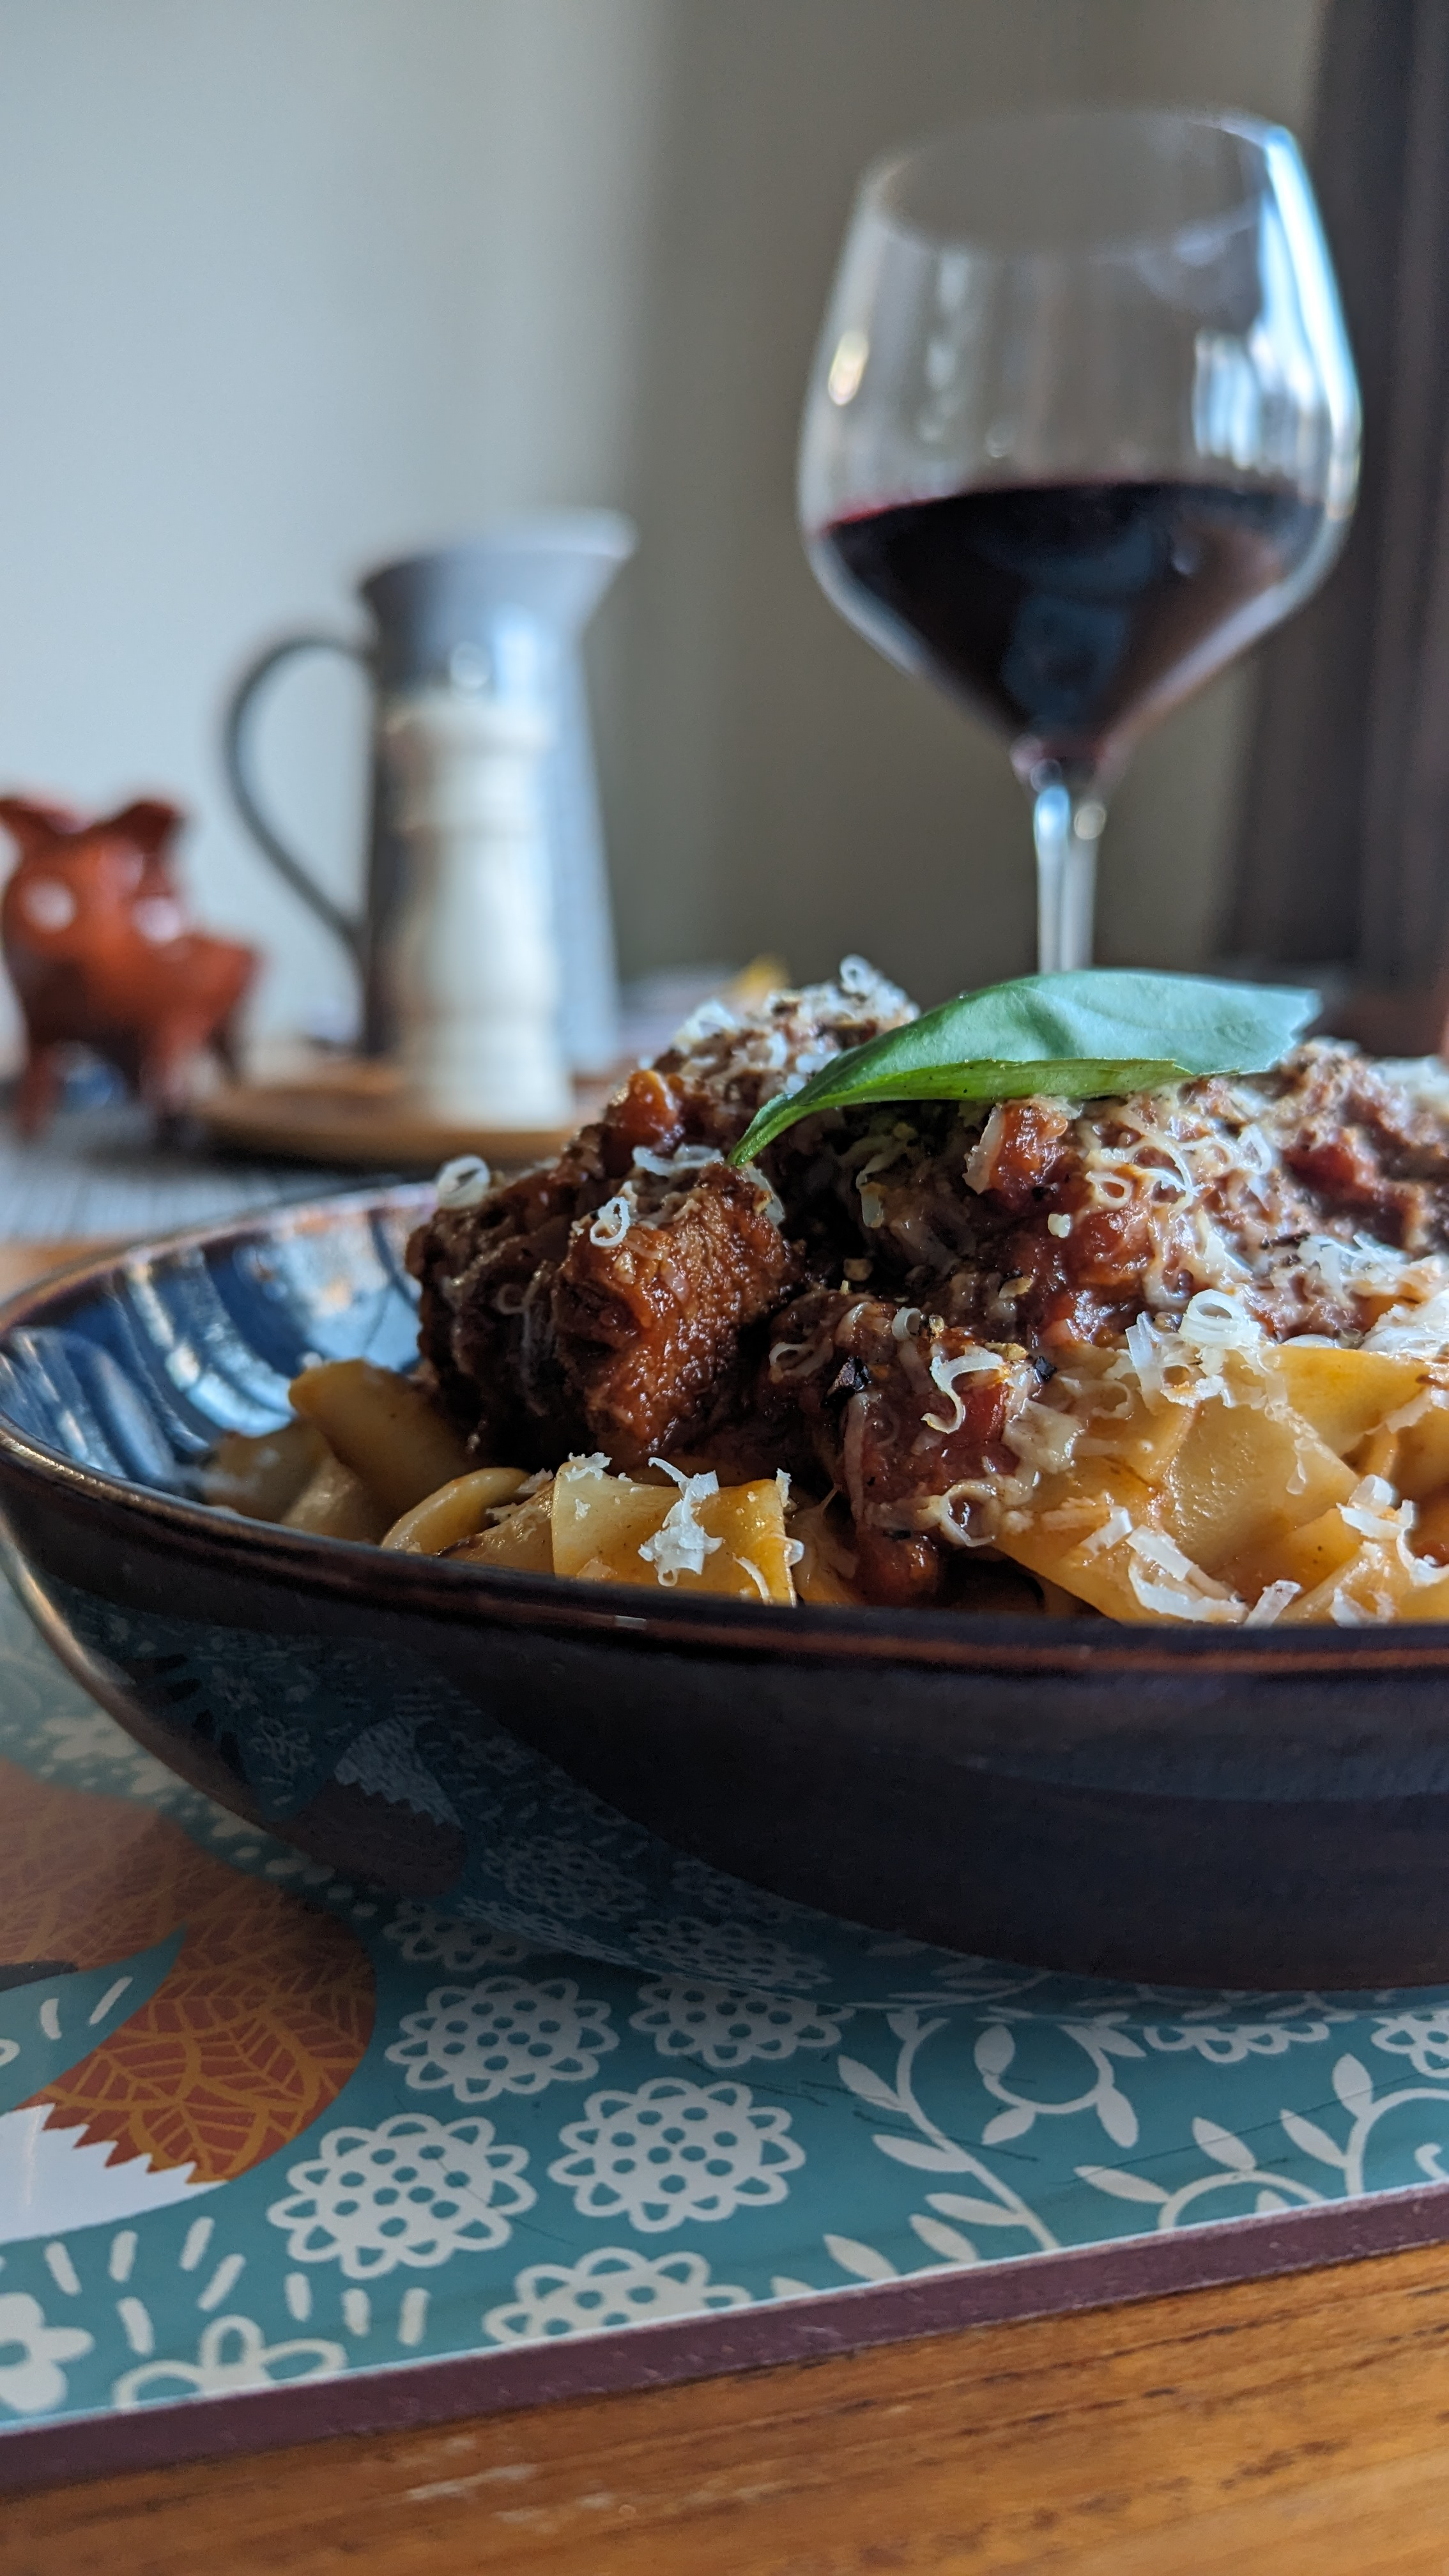
\includegraphics[width=\textwidth]{ragu}
      \column{0.33\textwidth}
      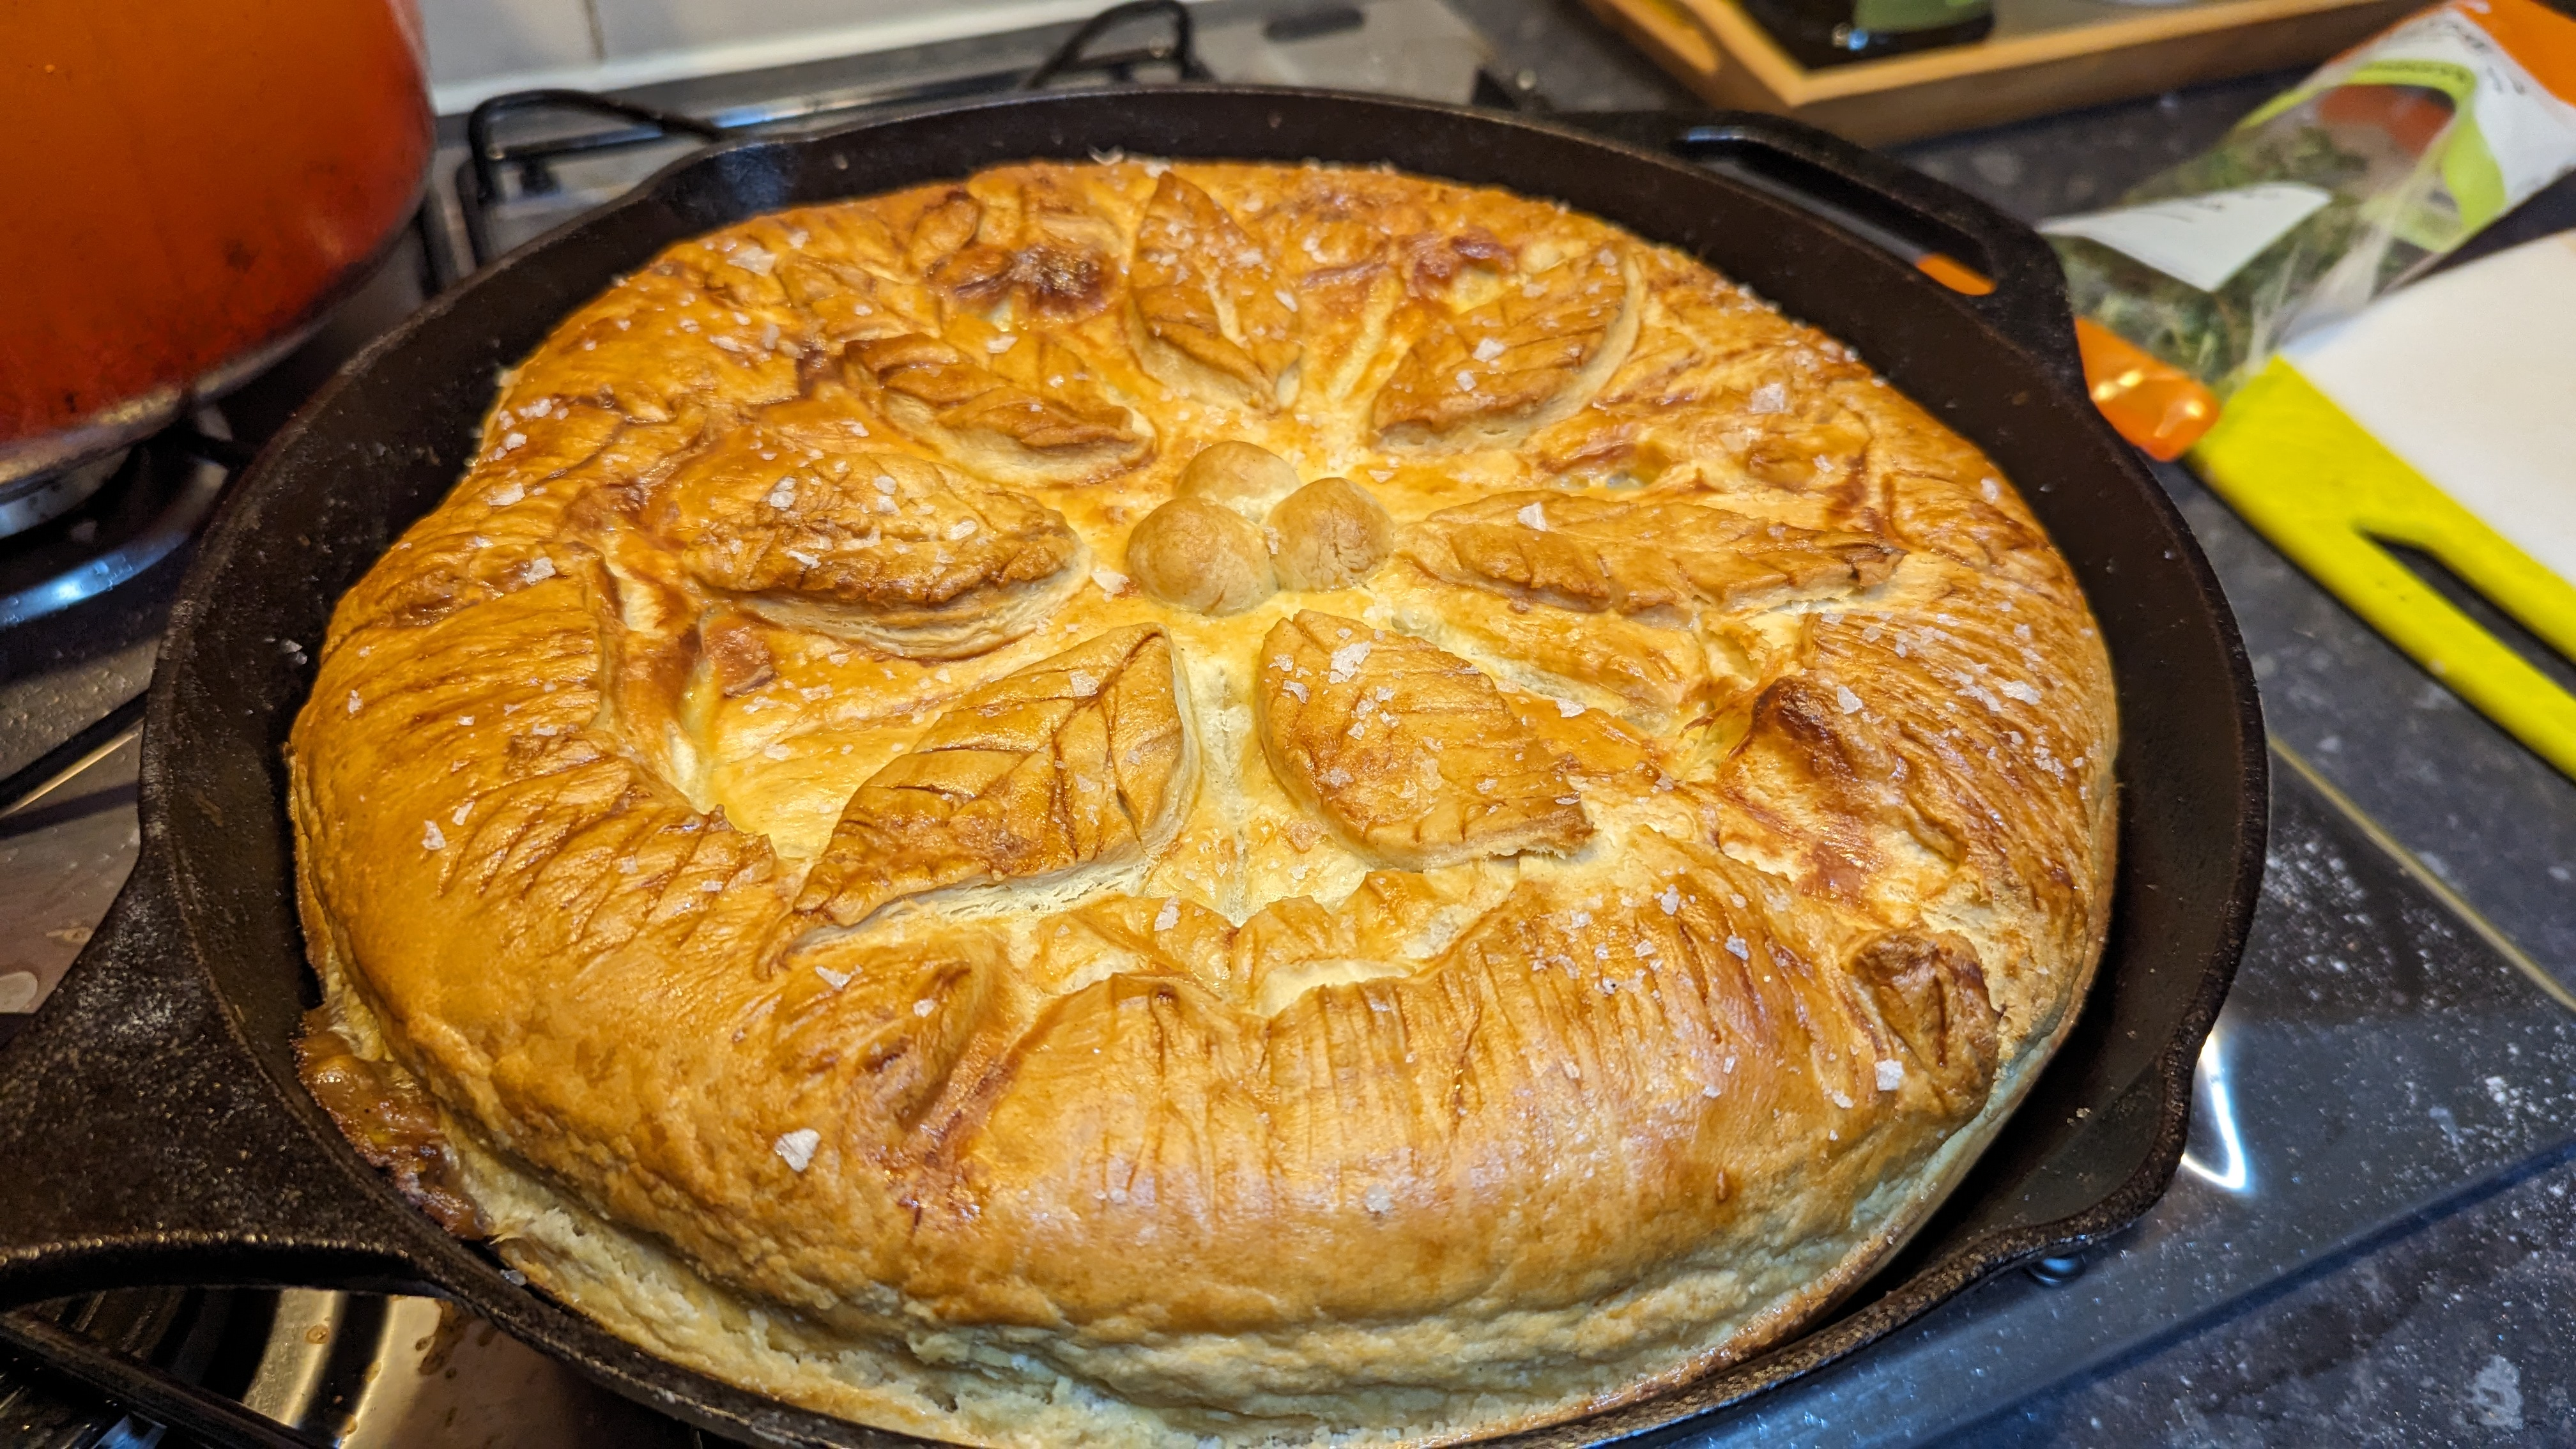
\includegraphics[width=\textwidth]{pie}\\
      \vspace{0.2cm}
      \includegraphics[width=\textwidth]{canard}\\
      \vspace{0.2cm}
      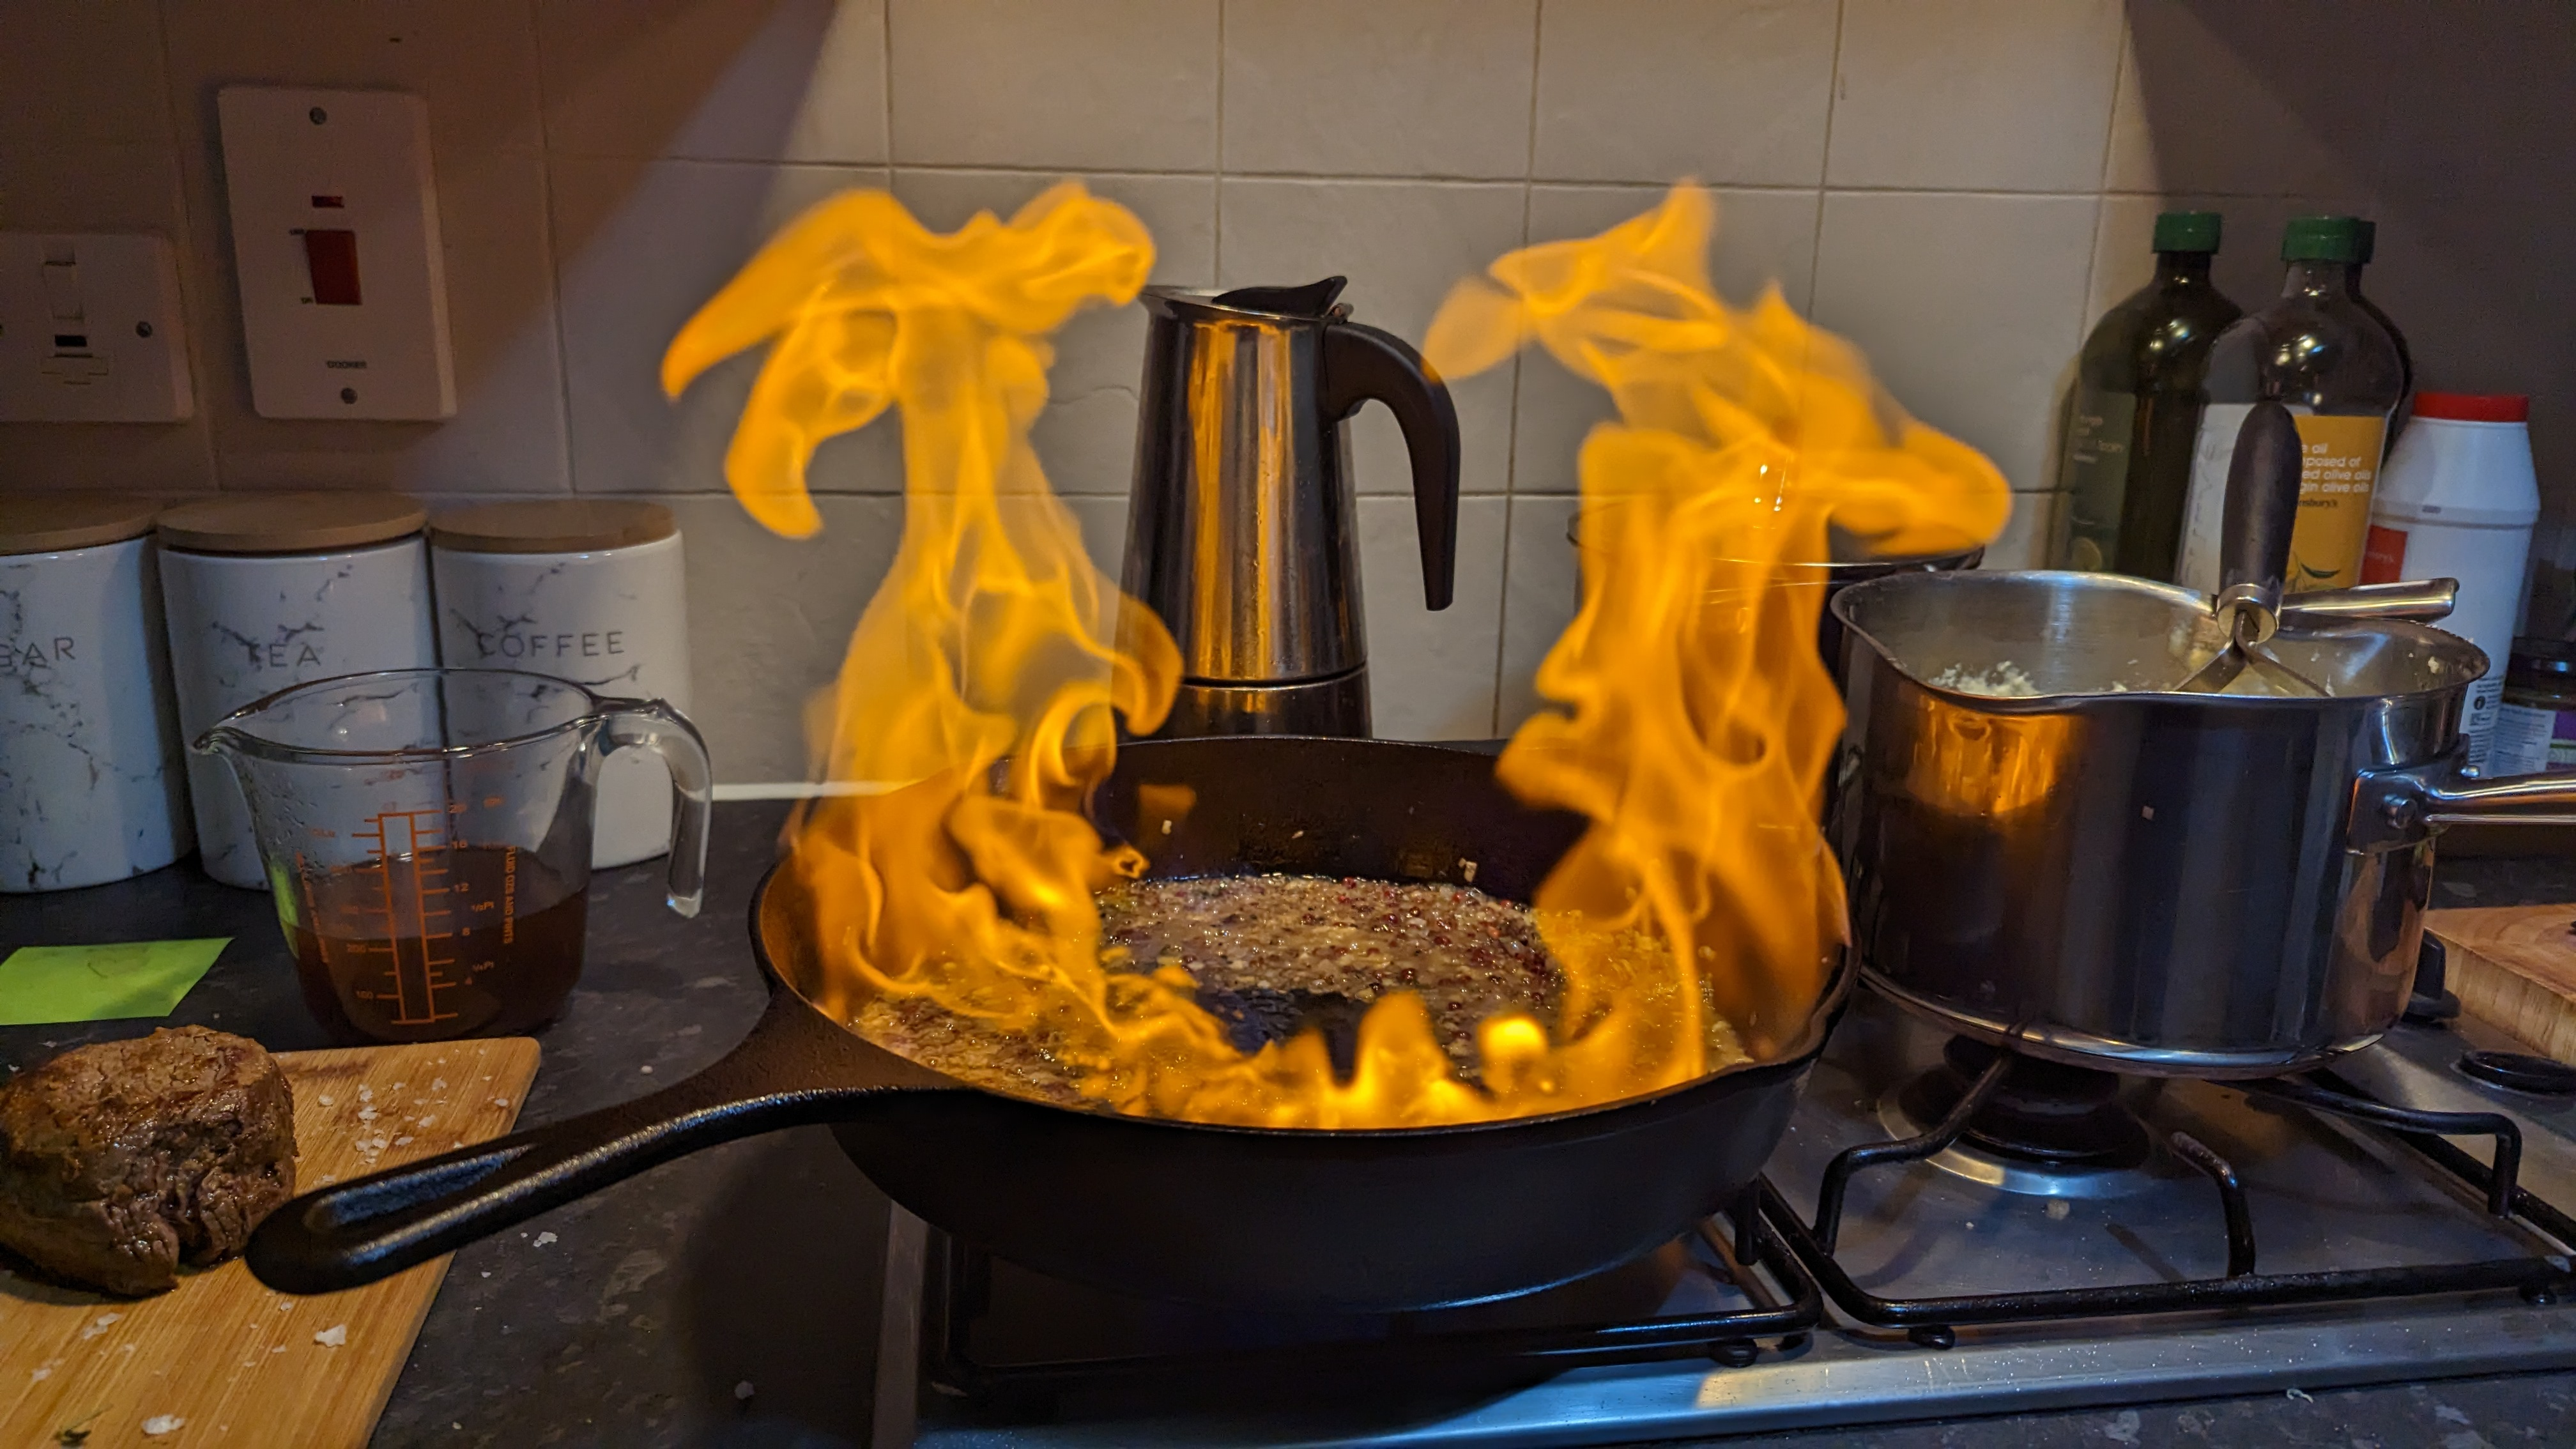
\includegraphics[width=\textwidth]{flambe}
    \end{columns}
  \end{frame}

  \begin{frame}{Out and About}
    \begin{columns}
      \column{0.5\textwidth}
        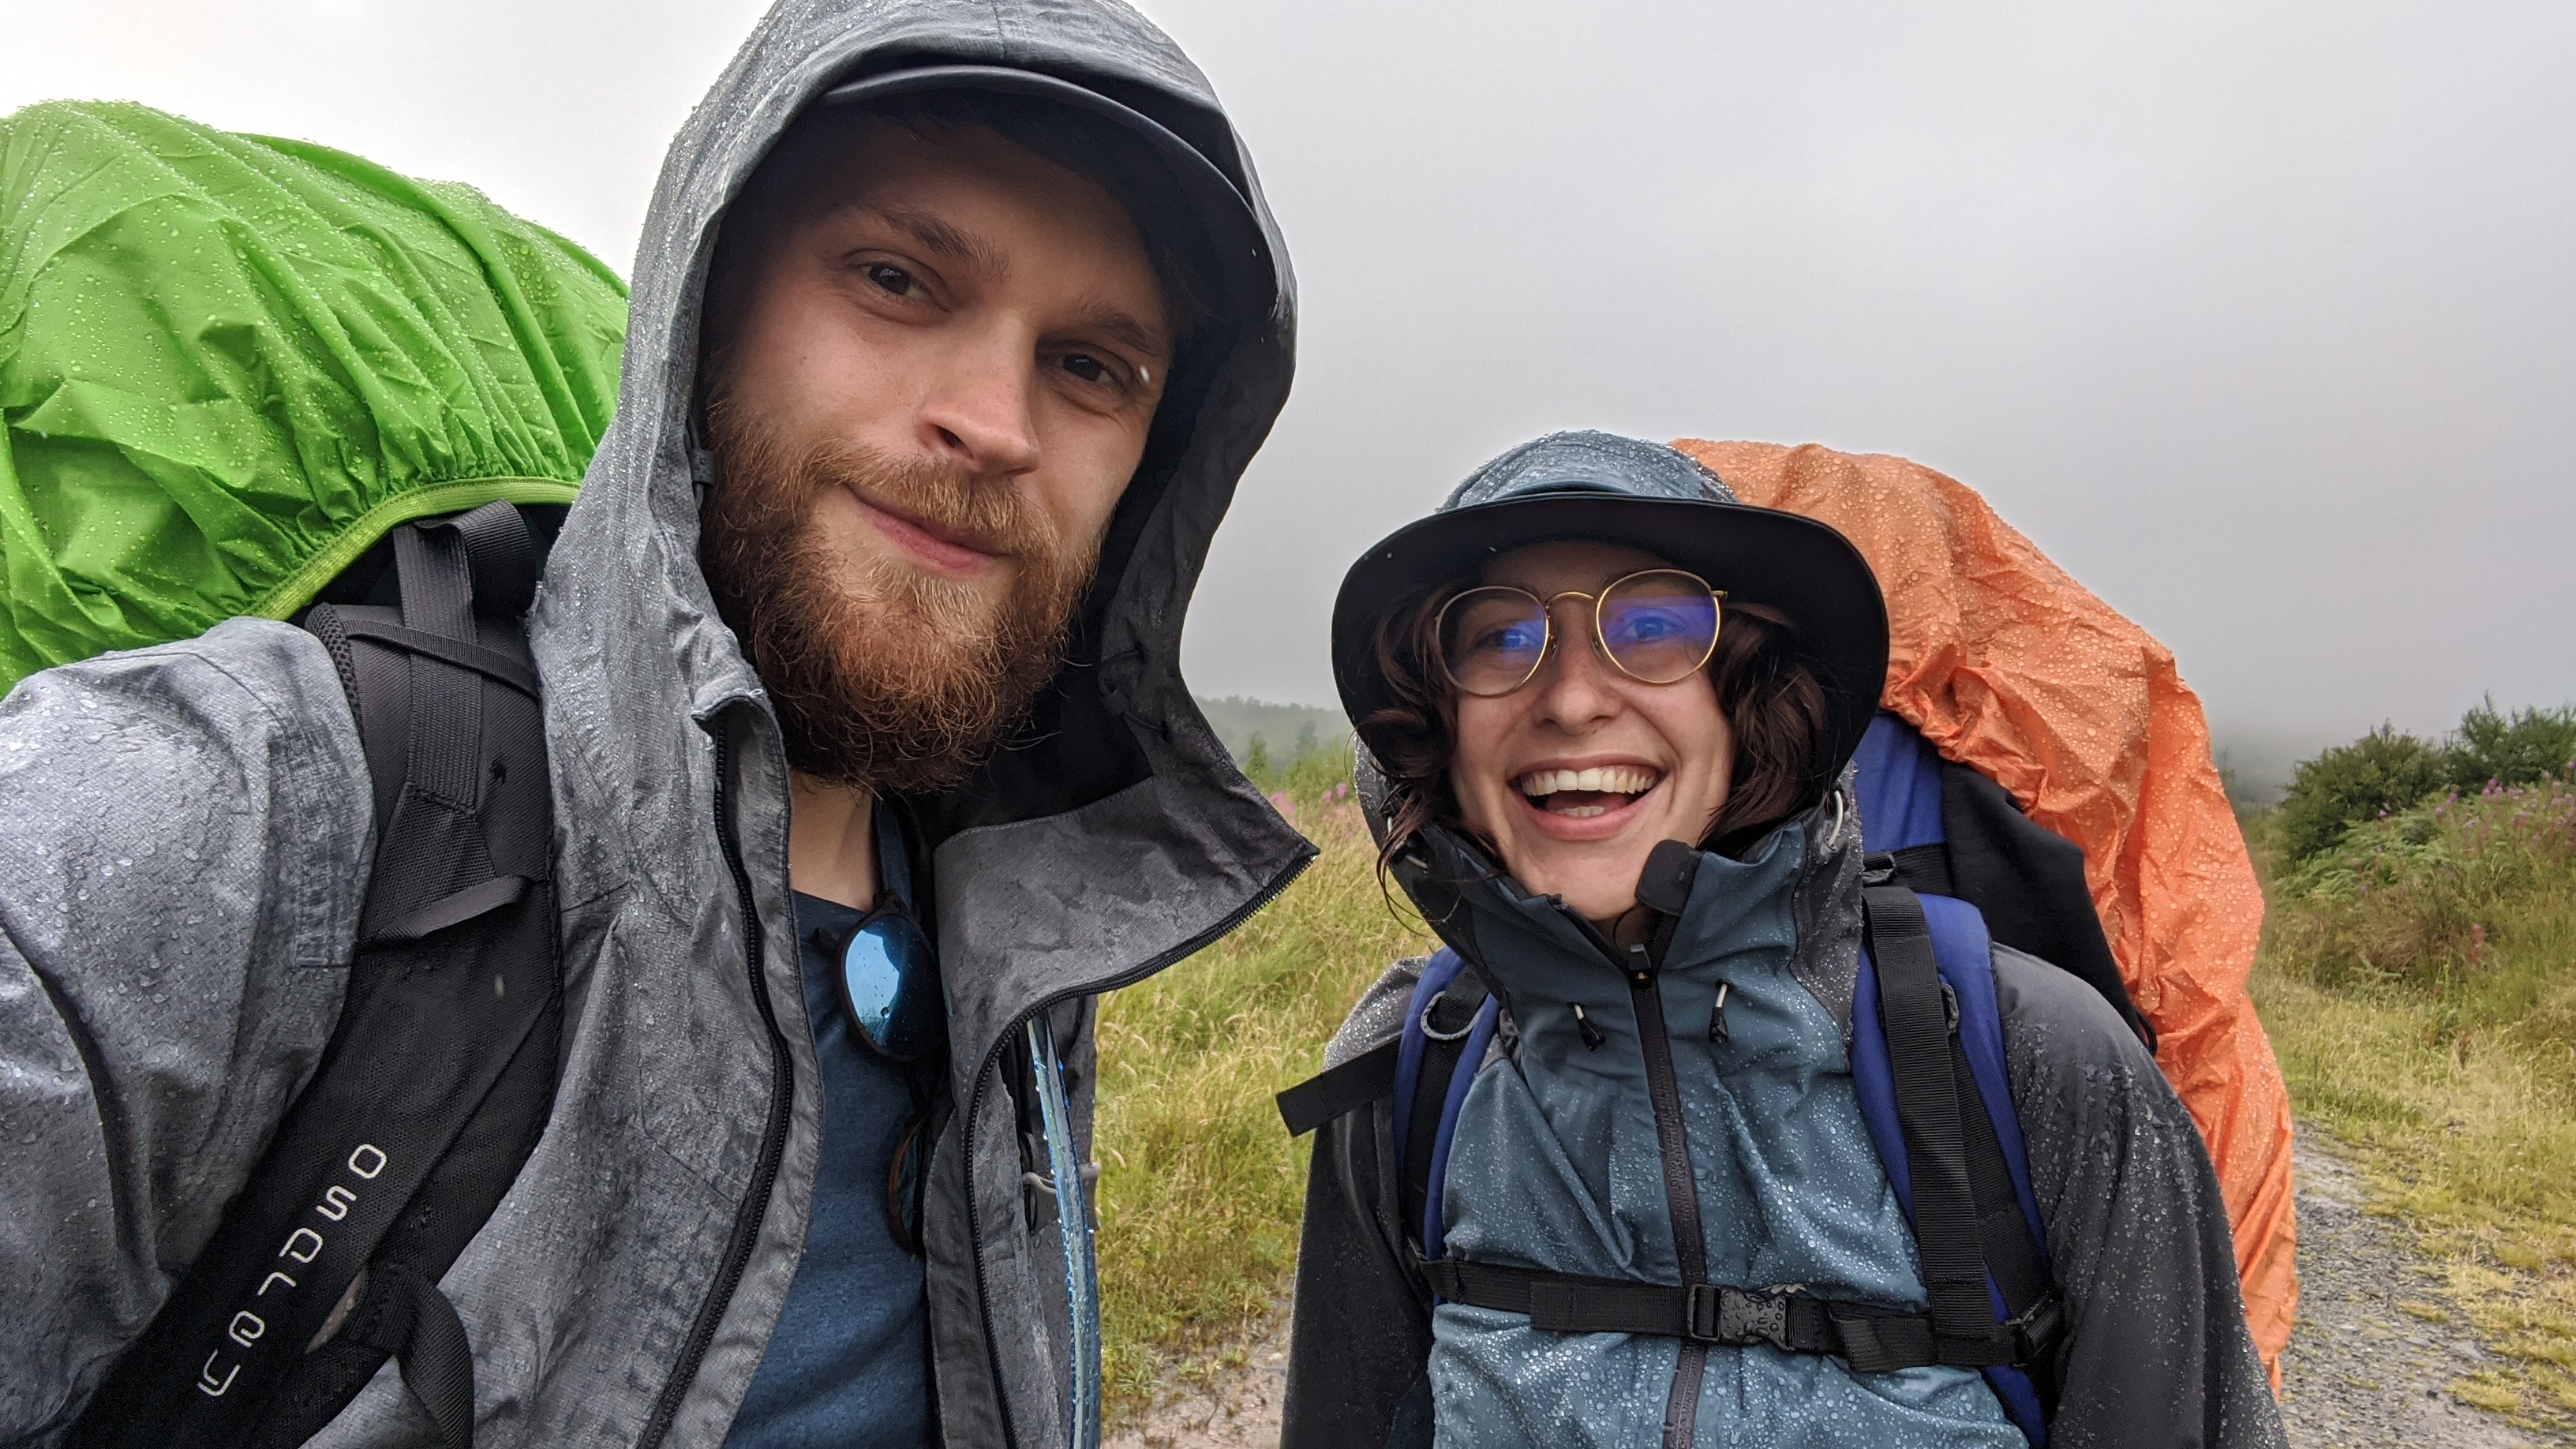
\includegraphics[width=\textwidth]{rain}\\
        \vspace{0.2cm}
        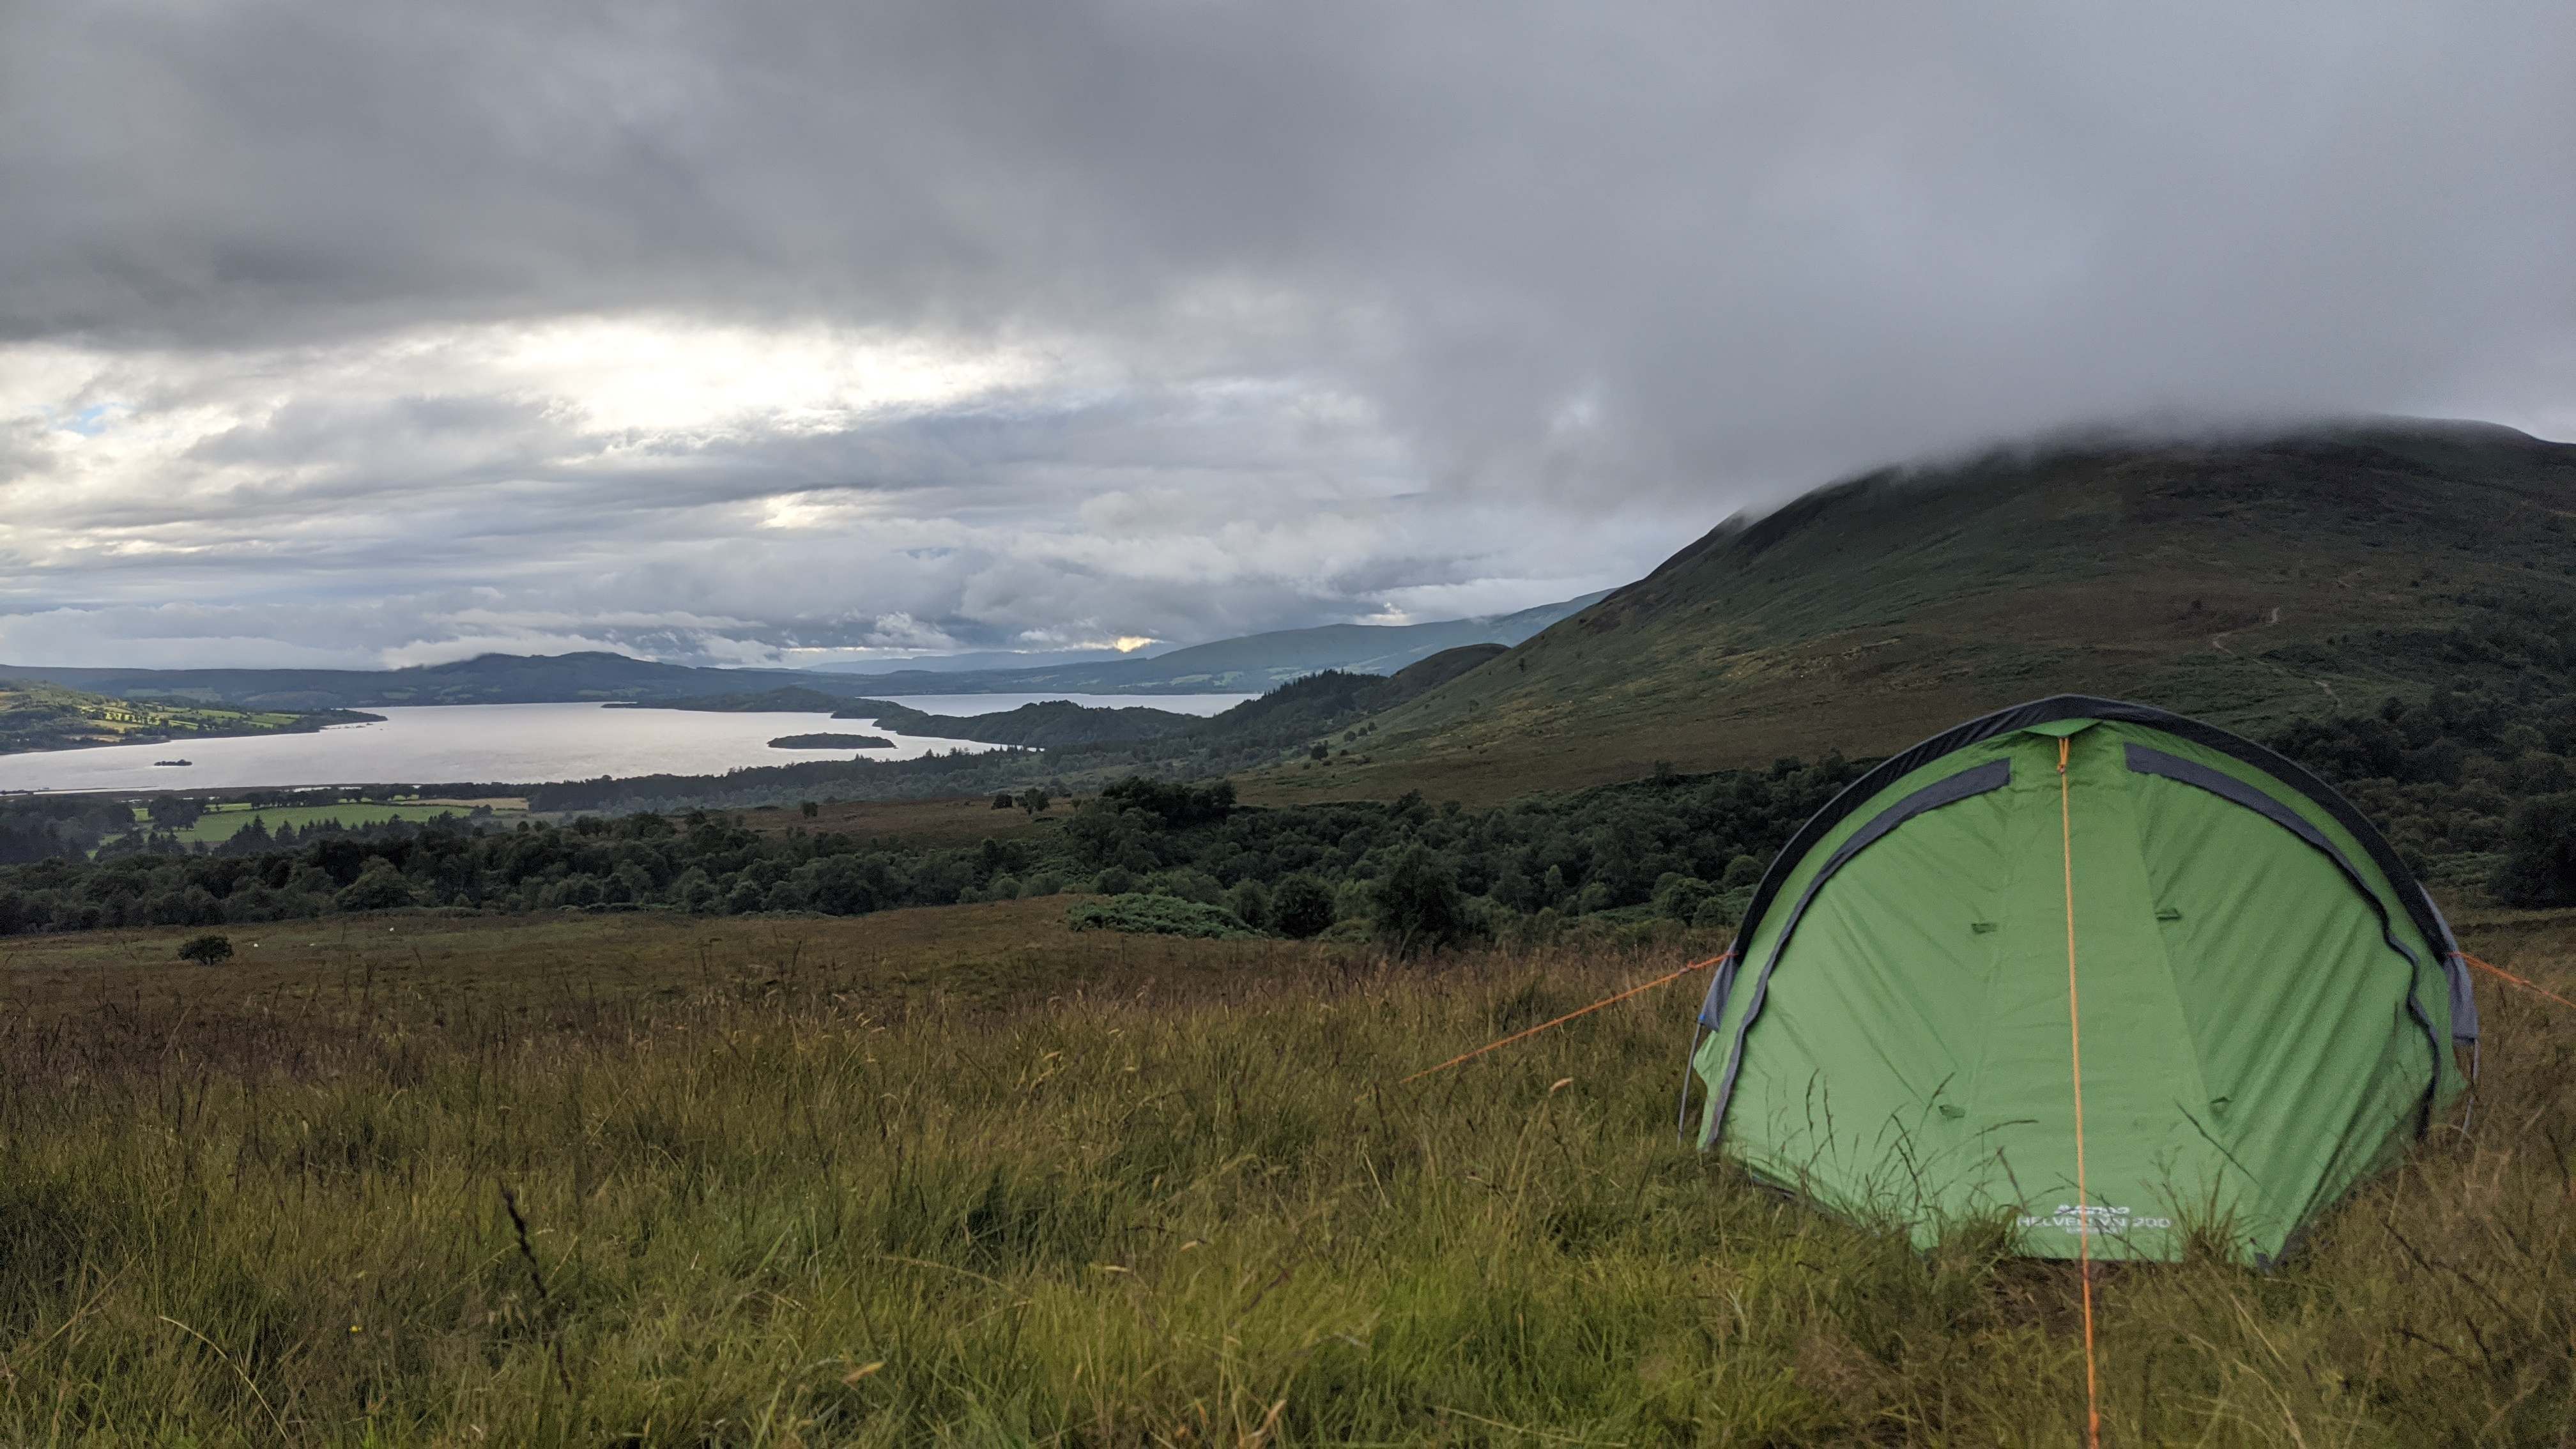
\includegraphics[width=\textwidth]{wild-camp}

      \column{0.5\textwidth}
        \includegraphics[width=\textwidth]{coo}\\
        \vspace{0.2cm}
        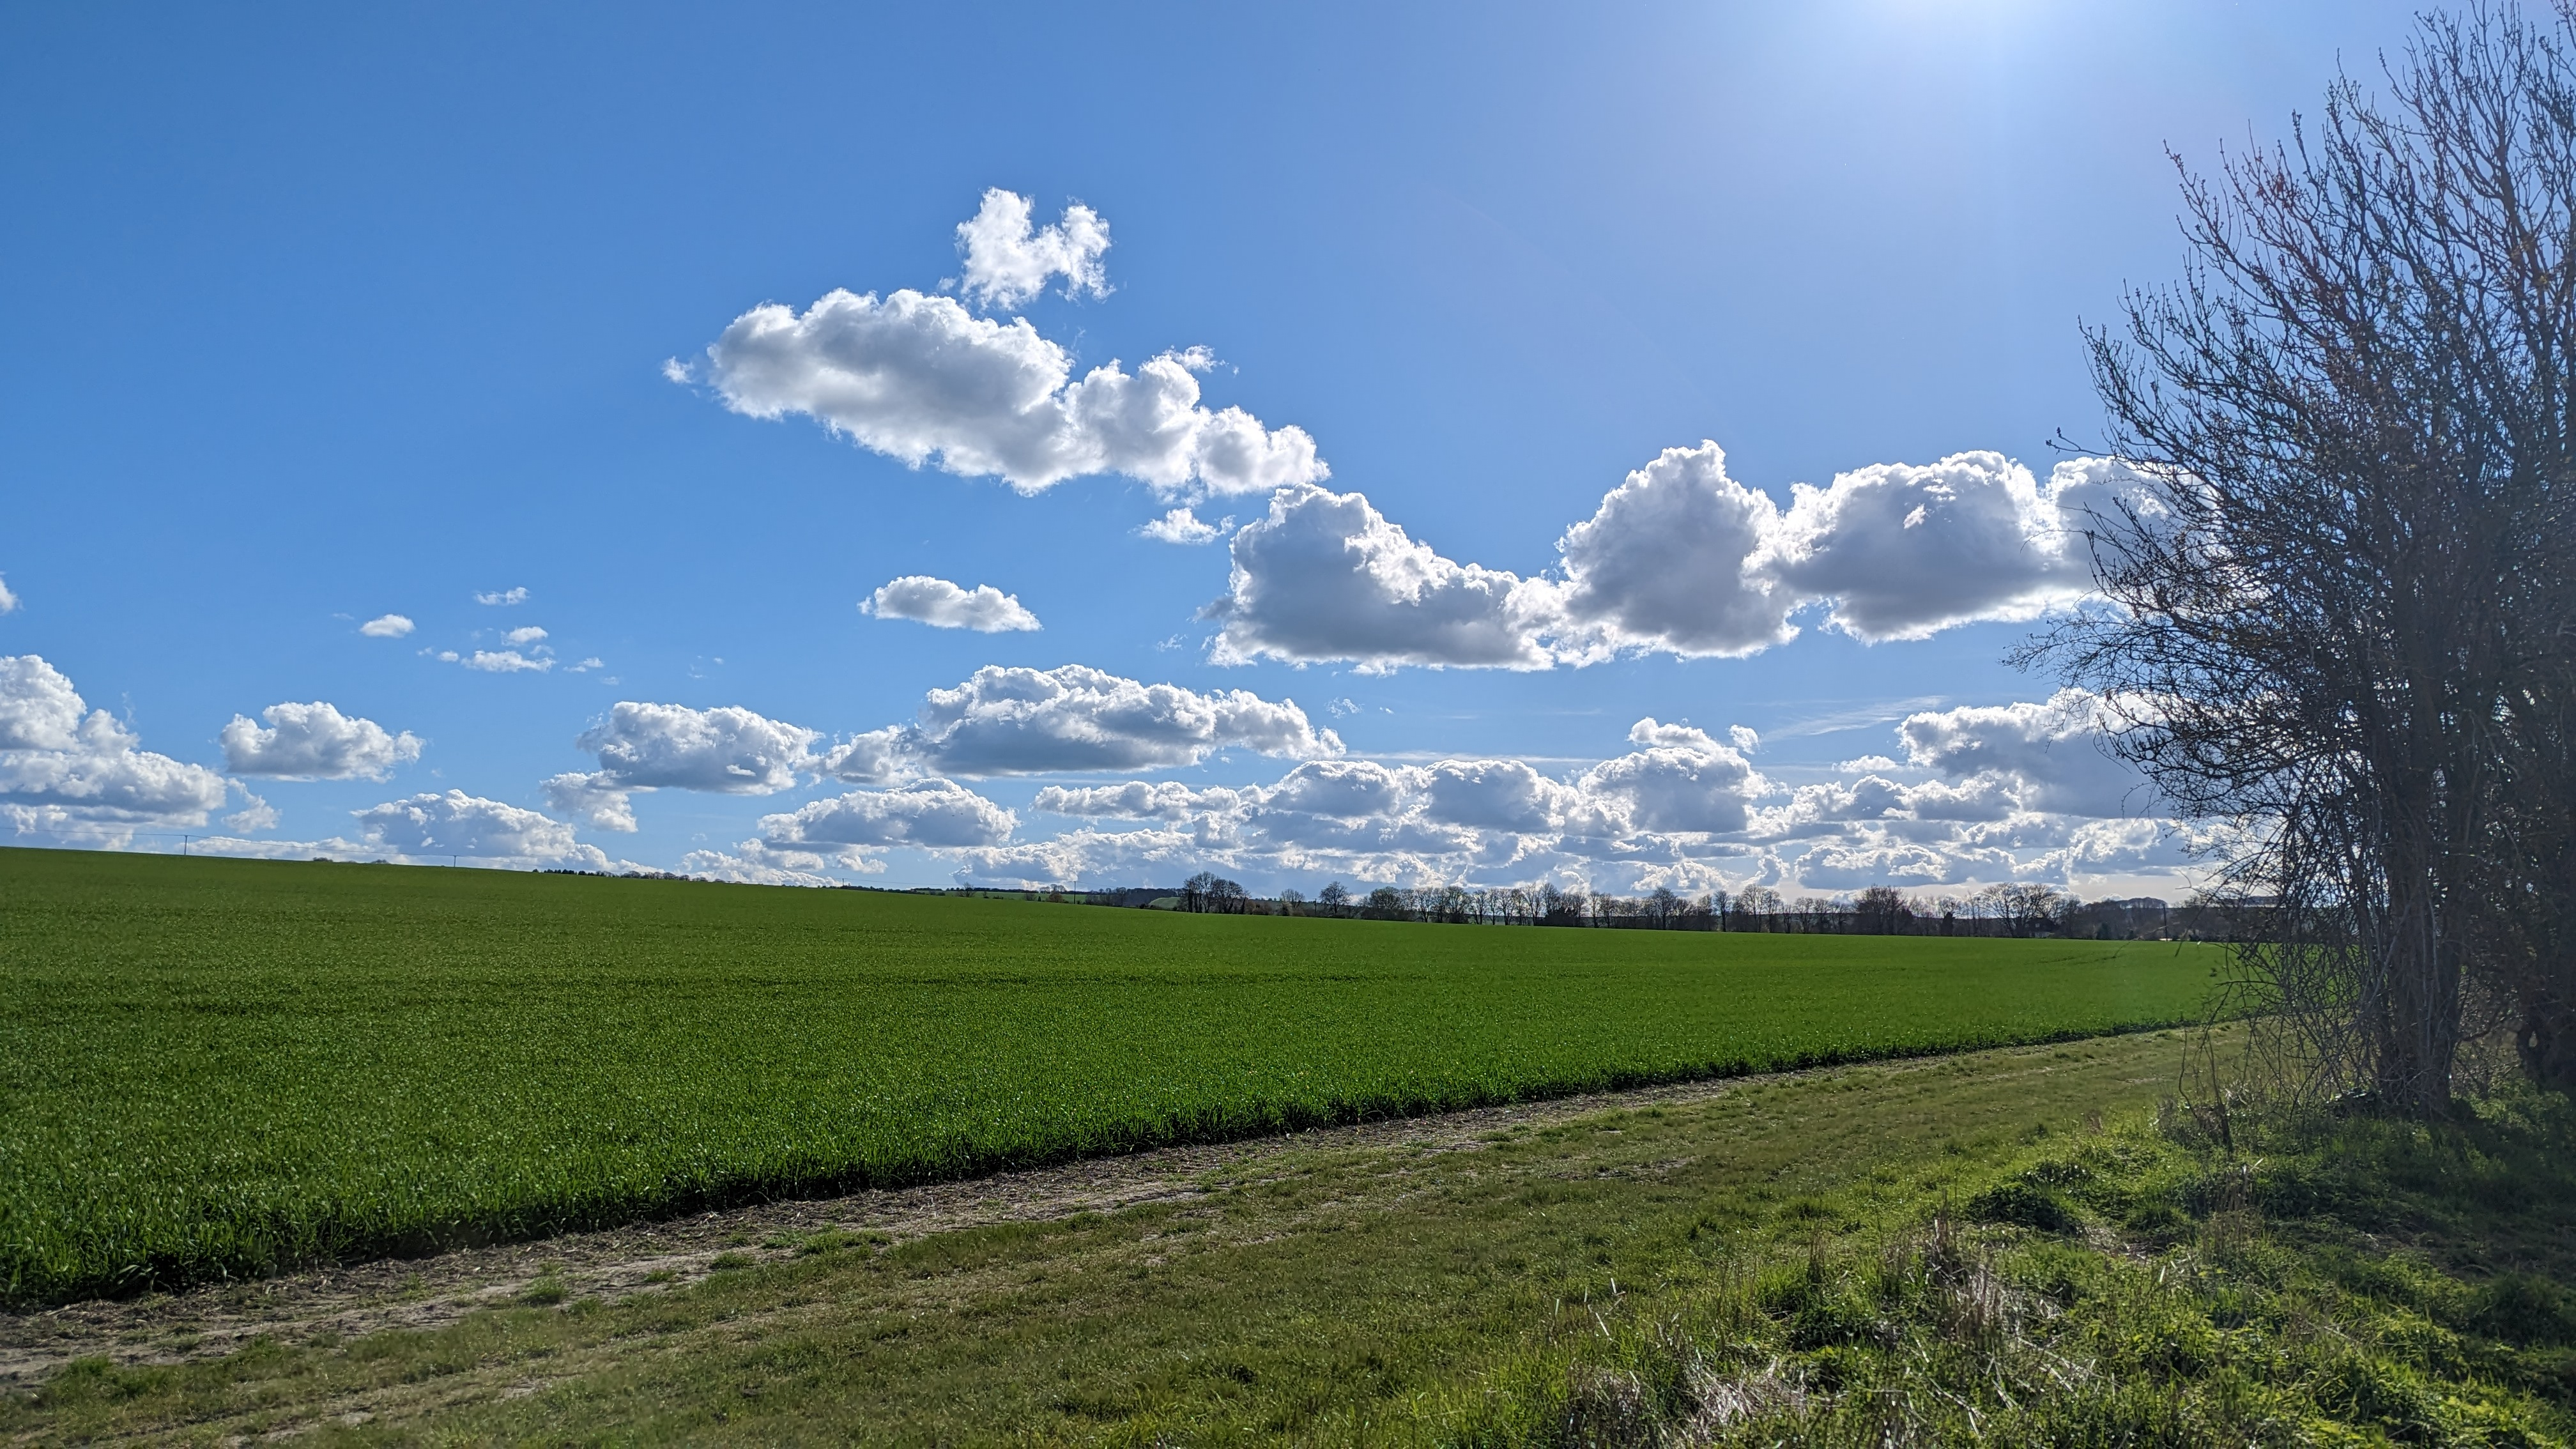
\includegraphics[width=\textwidth]{sunny}
    \end{columns}
  \end{frame}

  \begin{frame}{Admiring my Handiwork}
    \begin{columns}
      \column{0.5\textwidth}
        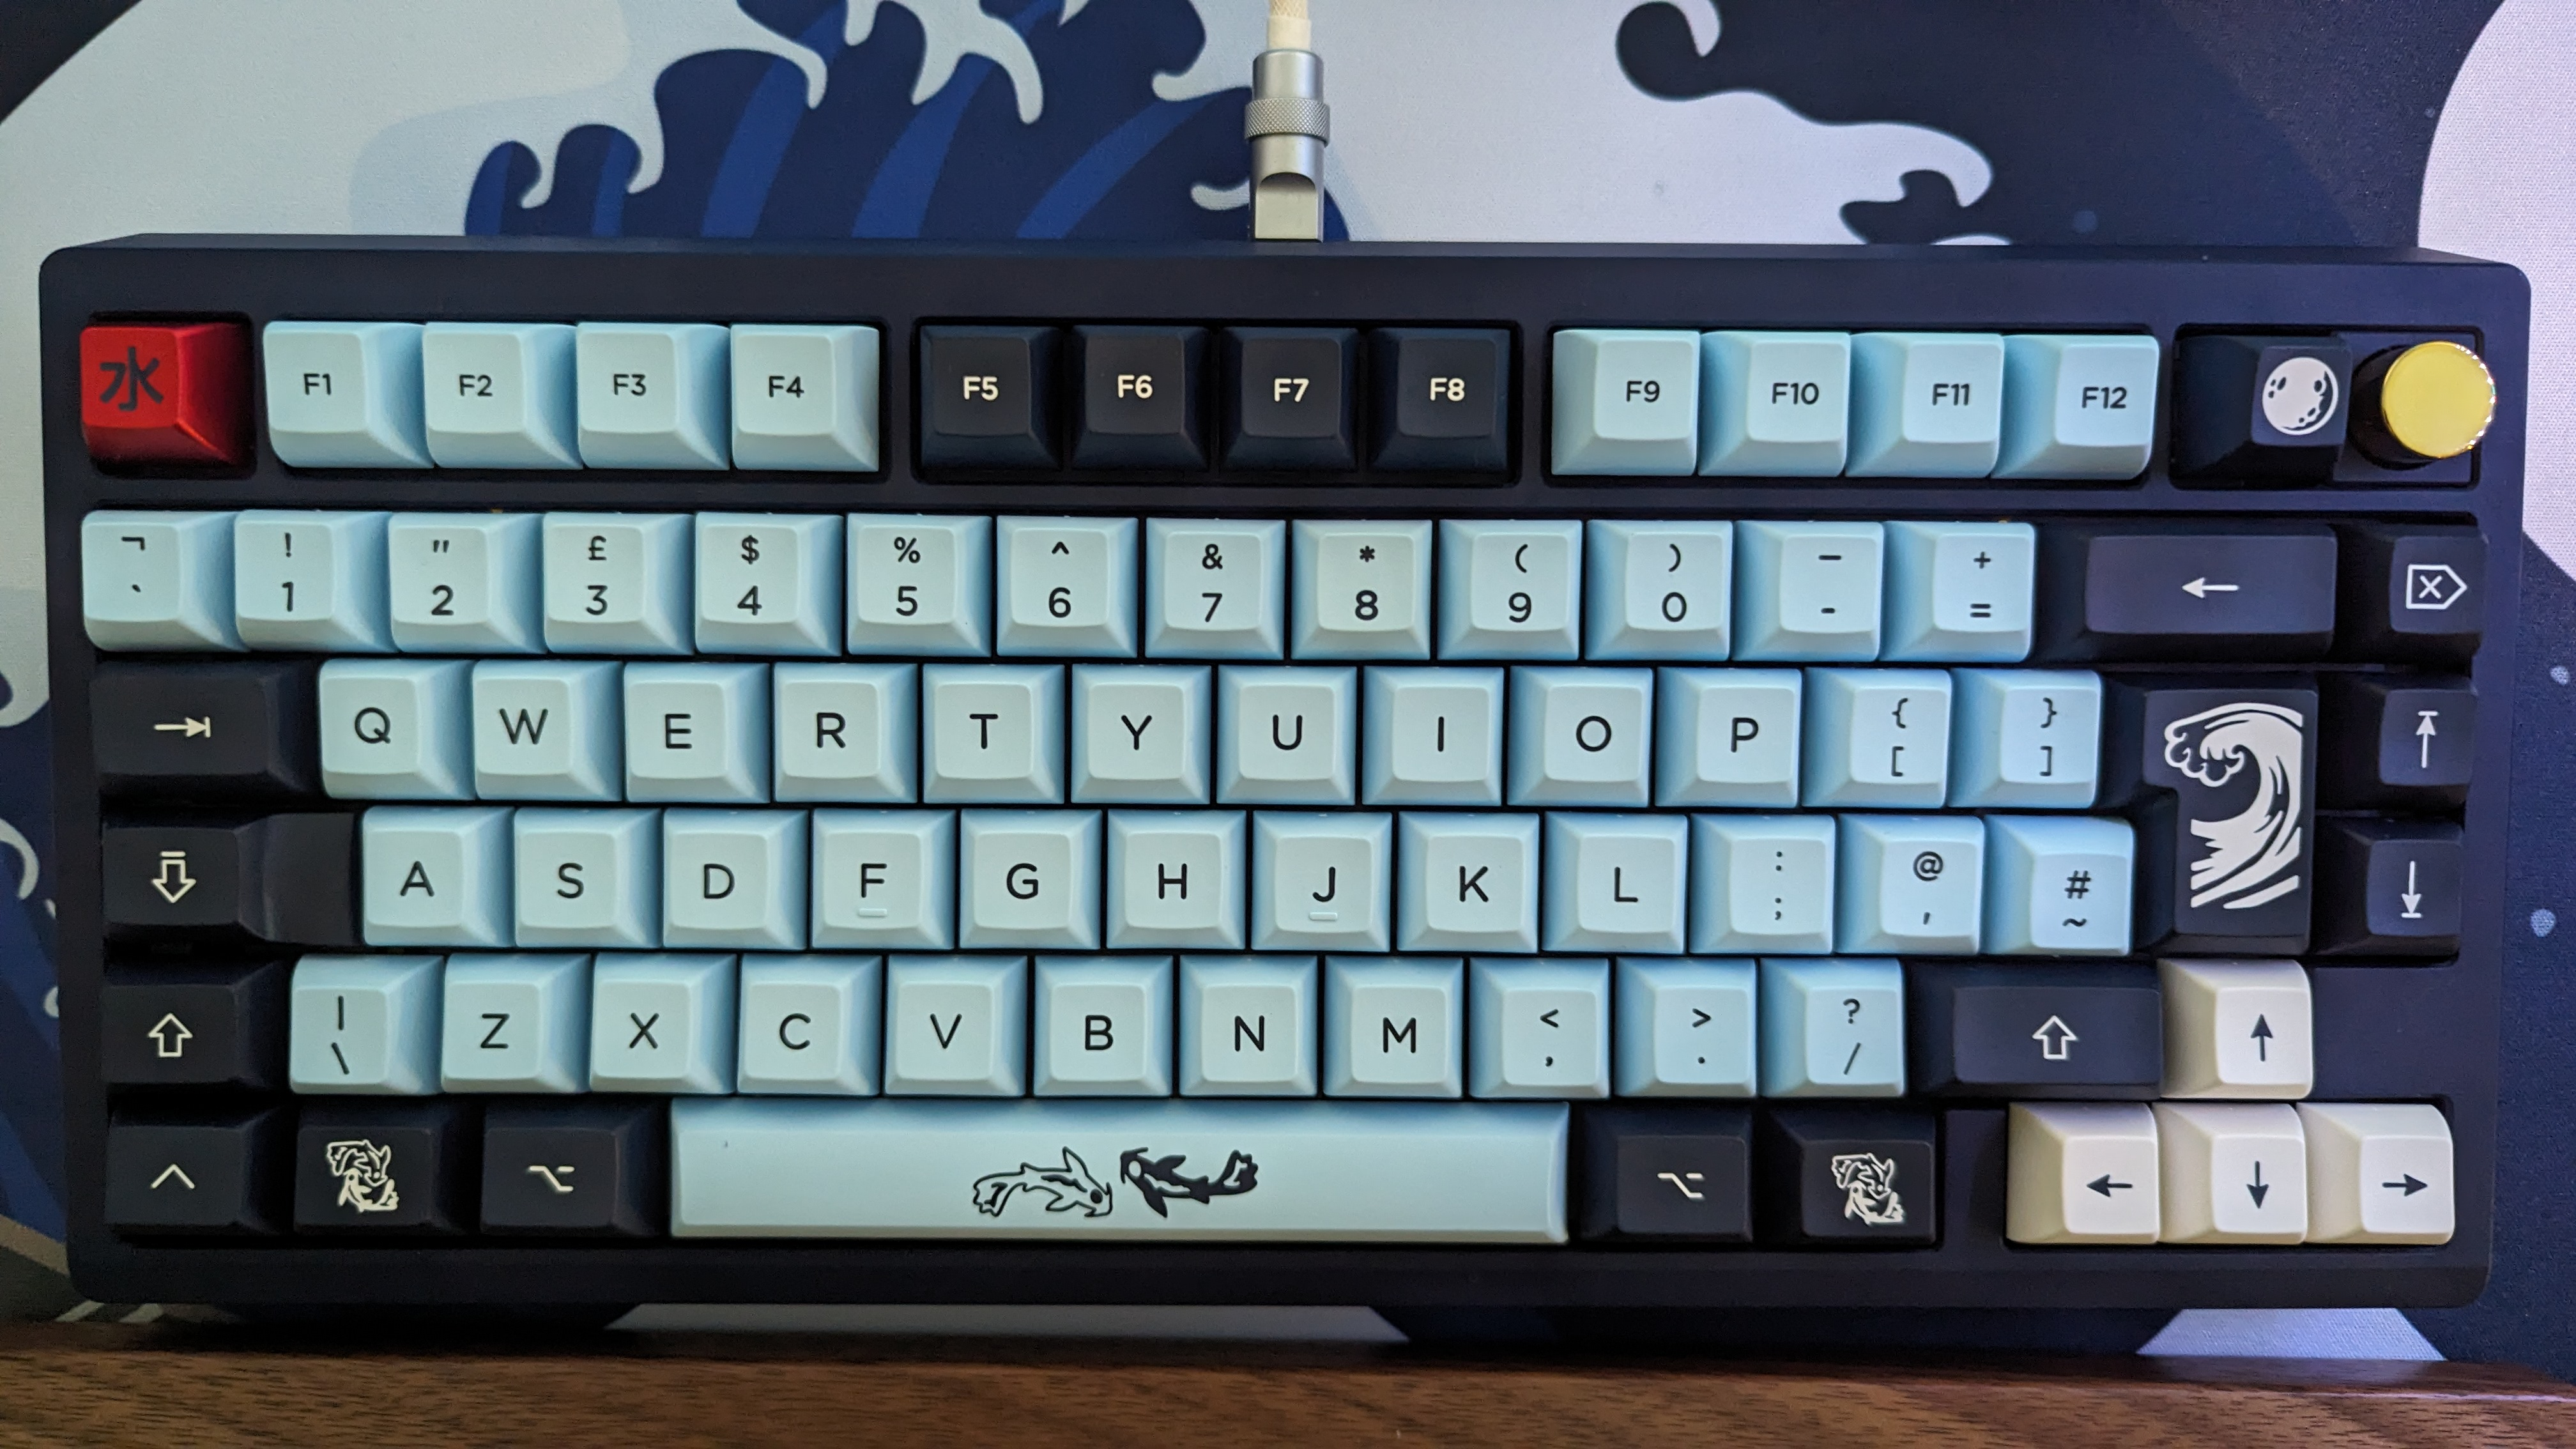
\includegraphics[width=\textwidth]{keyboard}\\
        \vspace{0.2cm}
        \includegraphics[width=\textwidth]{warhammer}

      \column{0.5\textwidth}
        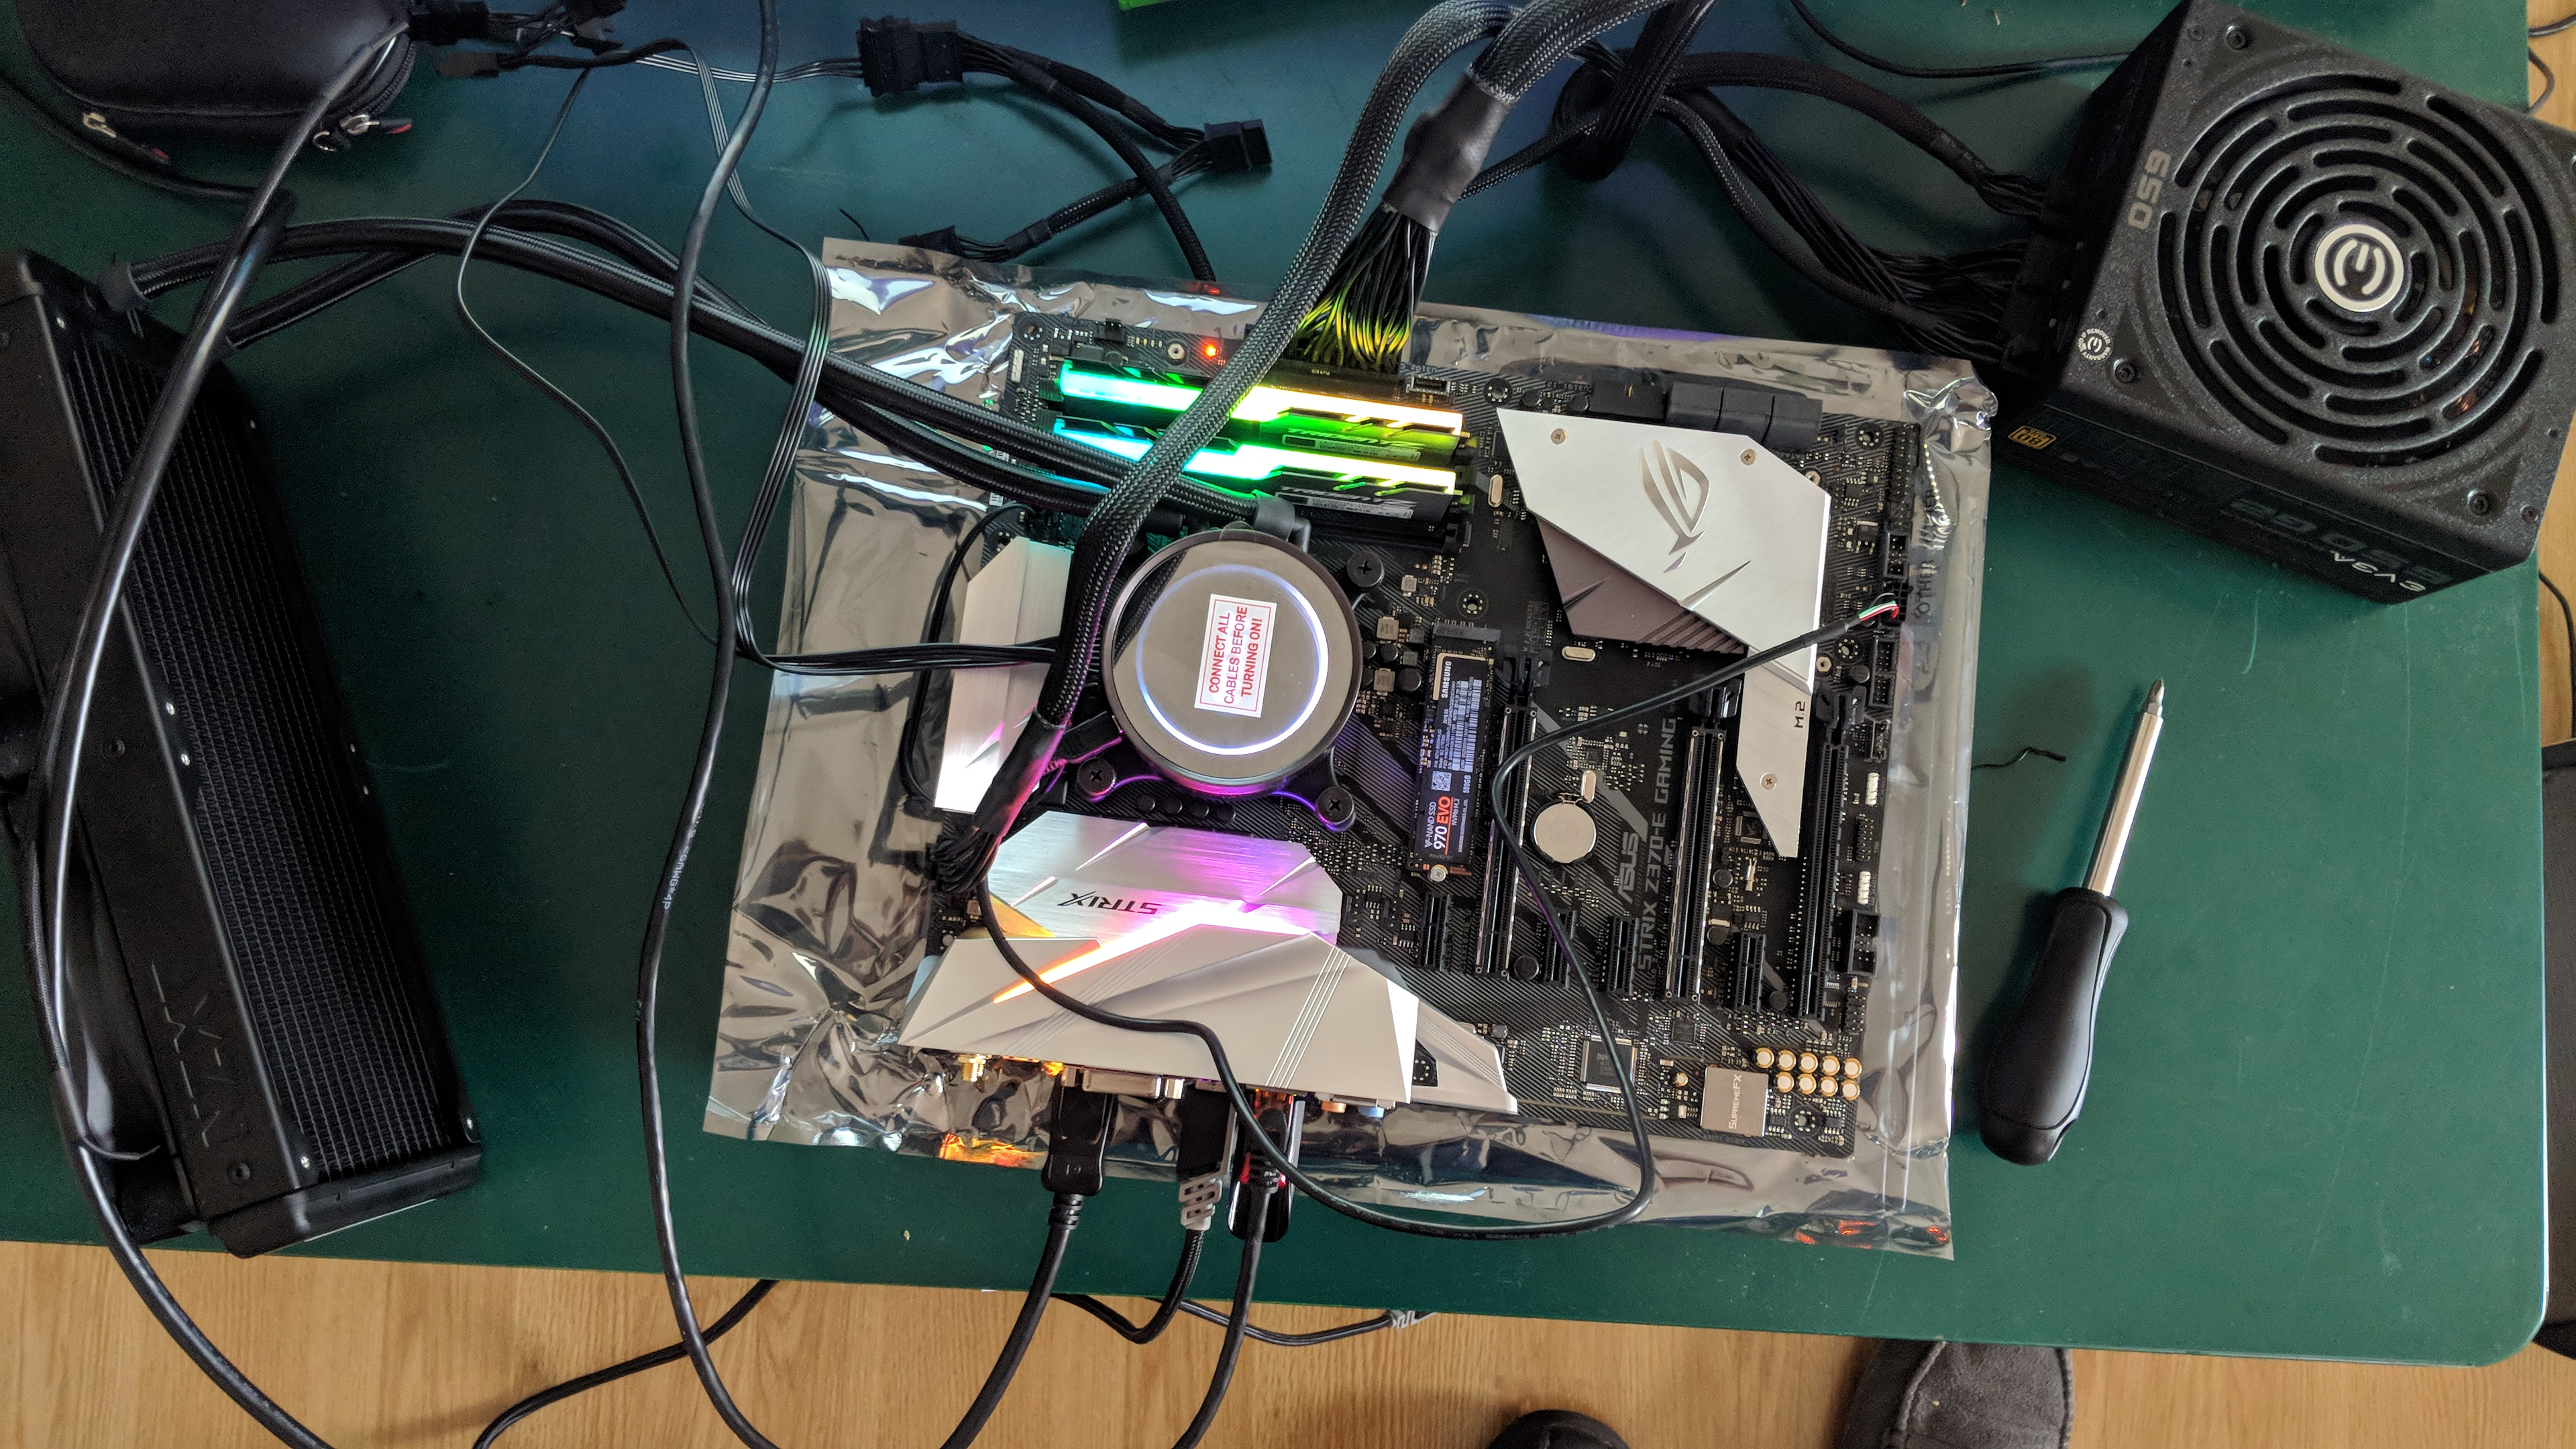
\includegraphics[width=\textwidth]{pc}\\
        \vspace{0.2cm}
        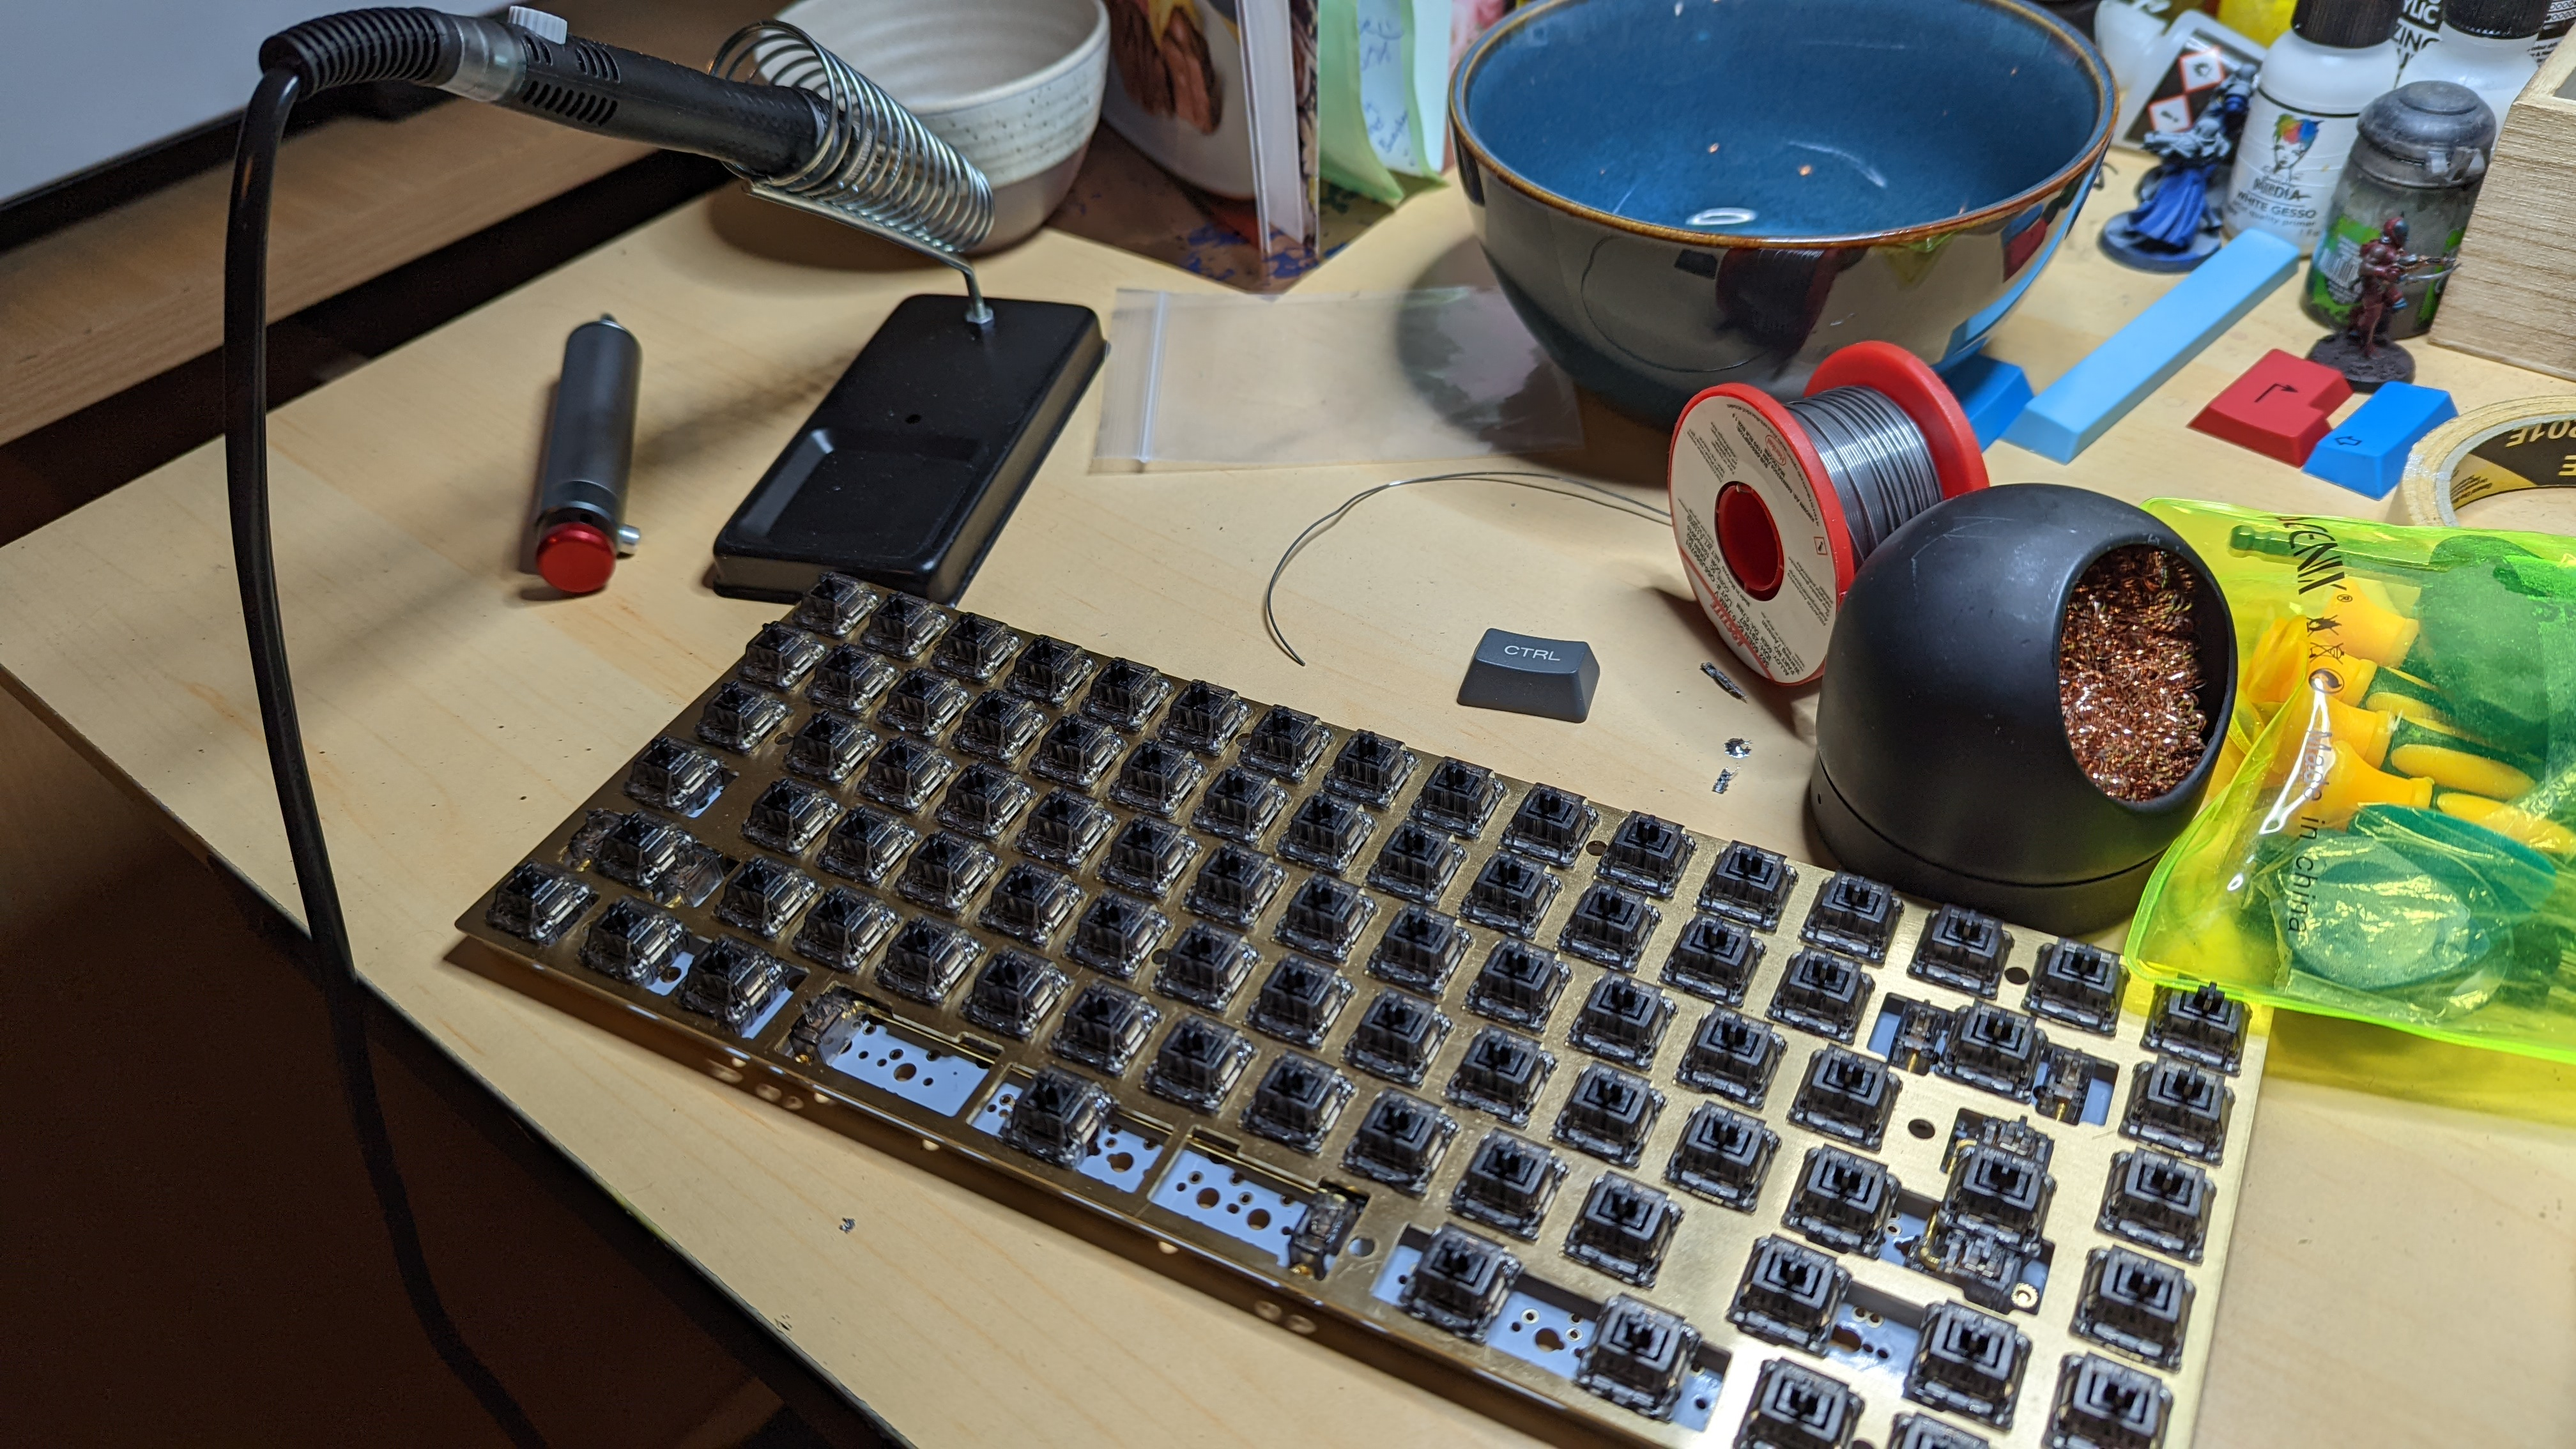
\includegraphics[width=\textwidth]{soldering}
    \end{columns}
  \end{frame}

  \section*{Thank you for listening!}
  \begin{frame}{Acknowledgements}
    \begin{itemize}
      \item \LaTeX Beamer theme. \footcite{mtheme}
    \end{itemize}
  \end{frame}

  \begin{frame}
    \printbibliography
  \end{frame}

\end{document}